\begin{apendicesenv}

\partapendices

\chapter{Pesquisa realizada}

Este apêndice apresenta o formulário realizado para as definições iniciais de qual sistema seria implementado no presente trabalho. As imagens anexadas contém as perguntas e as respostas dadas pelos possíveis usuários participantes da pesquisa.

\begin{figure}[h]
	\centering
	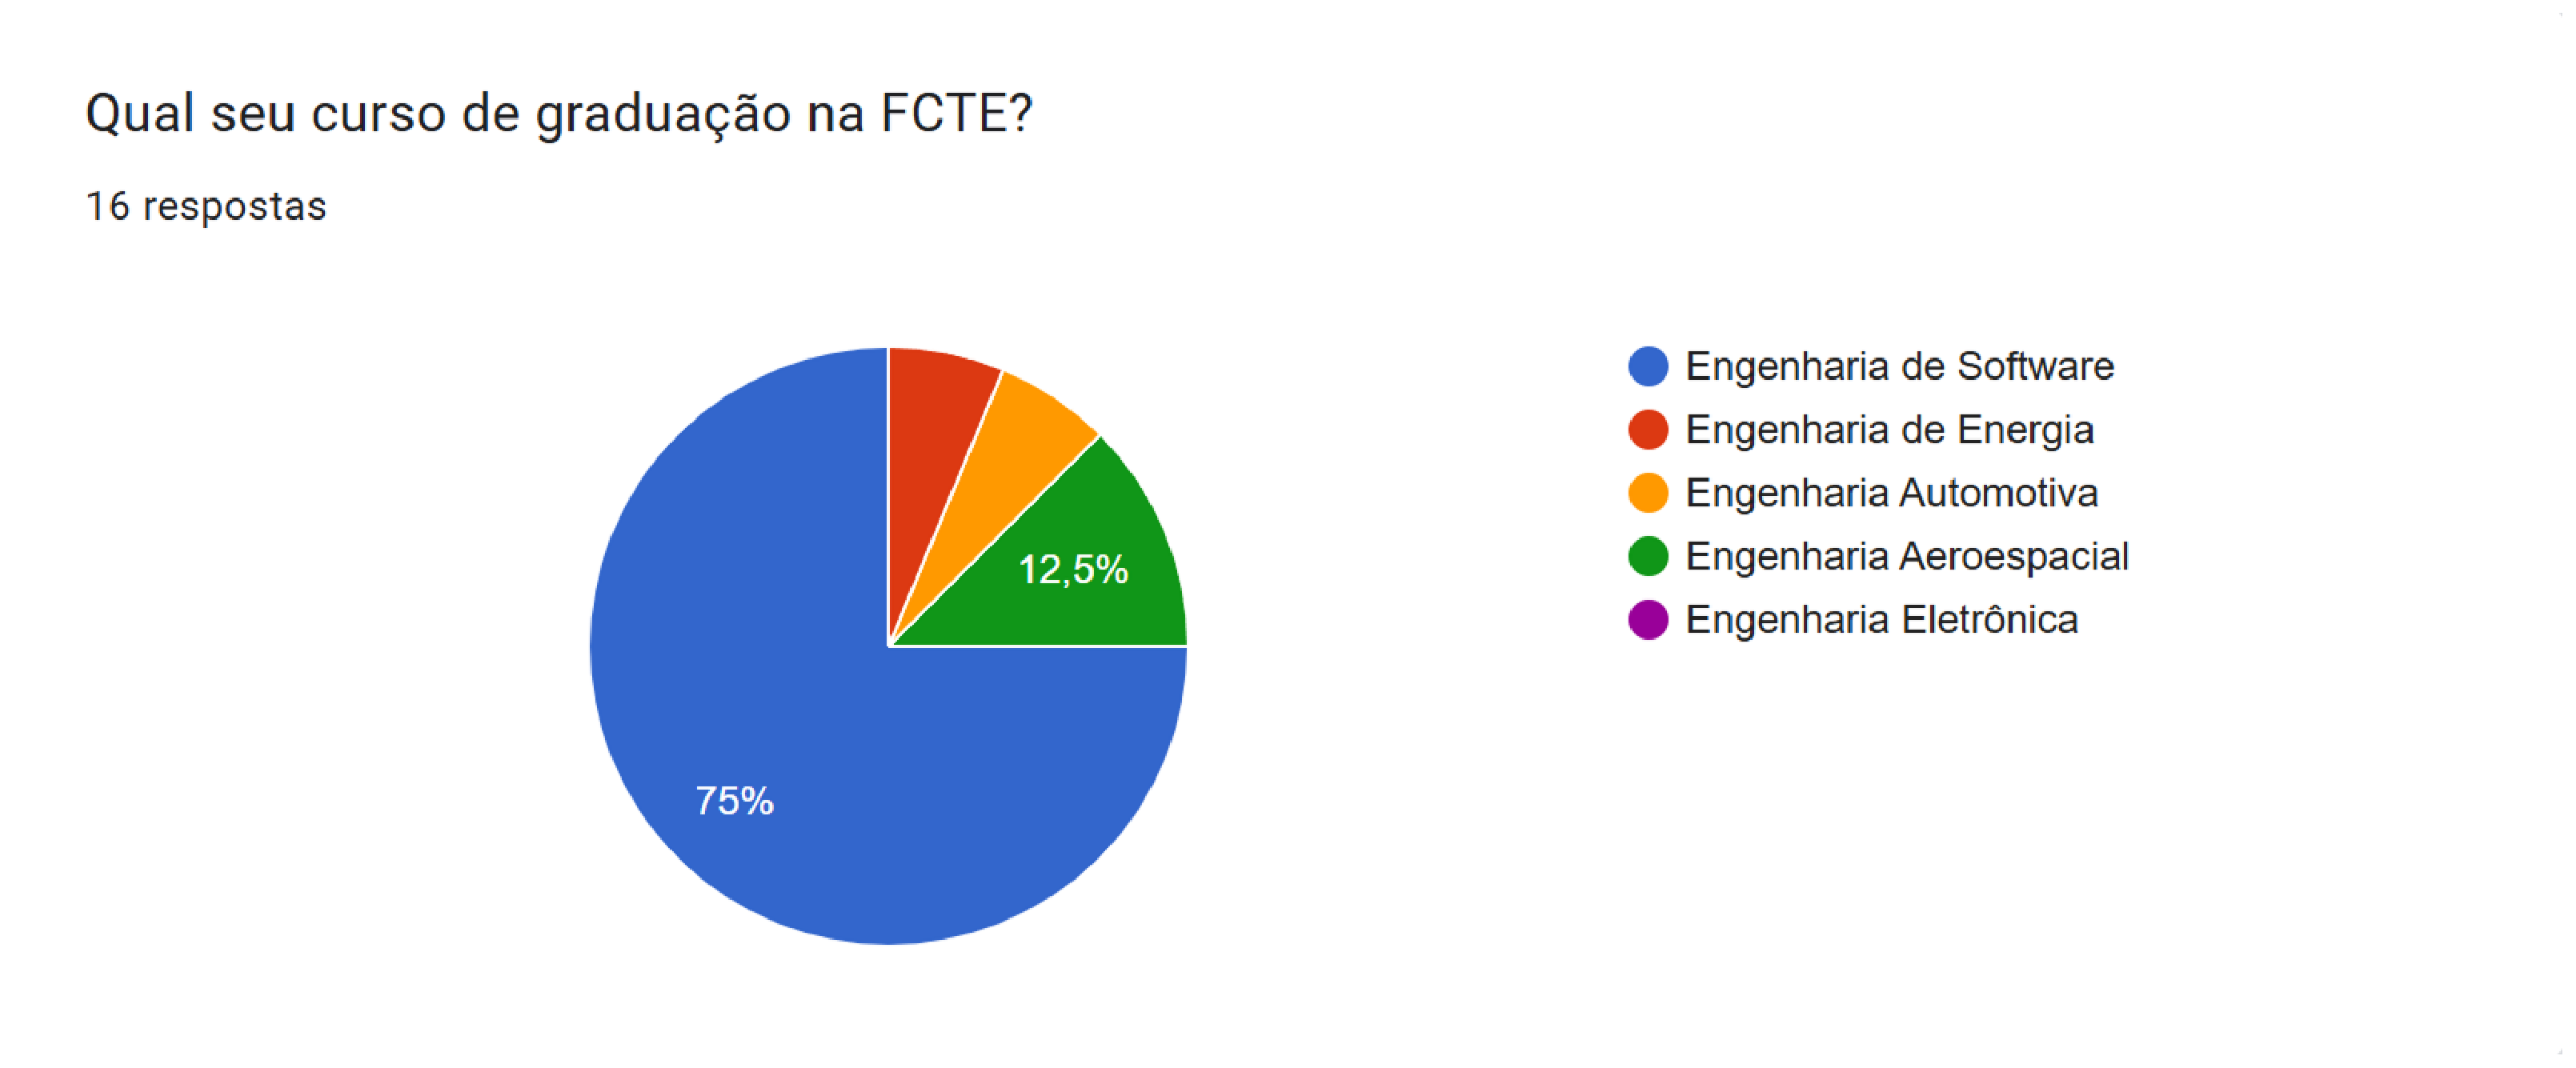
\includegraphics[width=1\linewidth]{./figuras/S1P1.eps}
	\caption{Seção 1 - Pergunta 1}
	\footnotesize Fonte: Autores.
	\label{fig06}
\end{figure}

\begin{figure}[h]
	\centering
	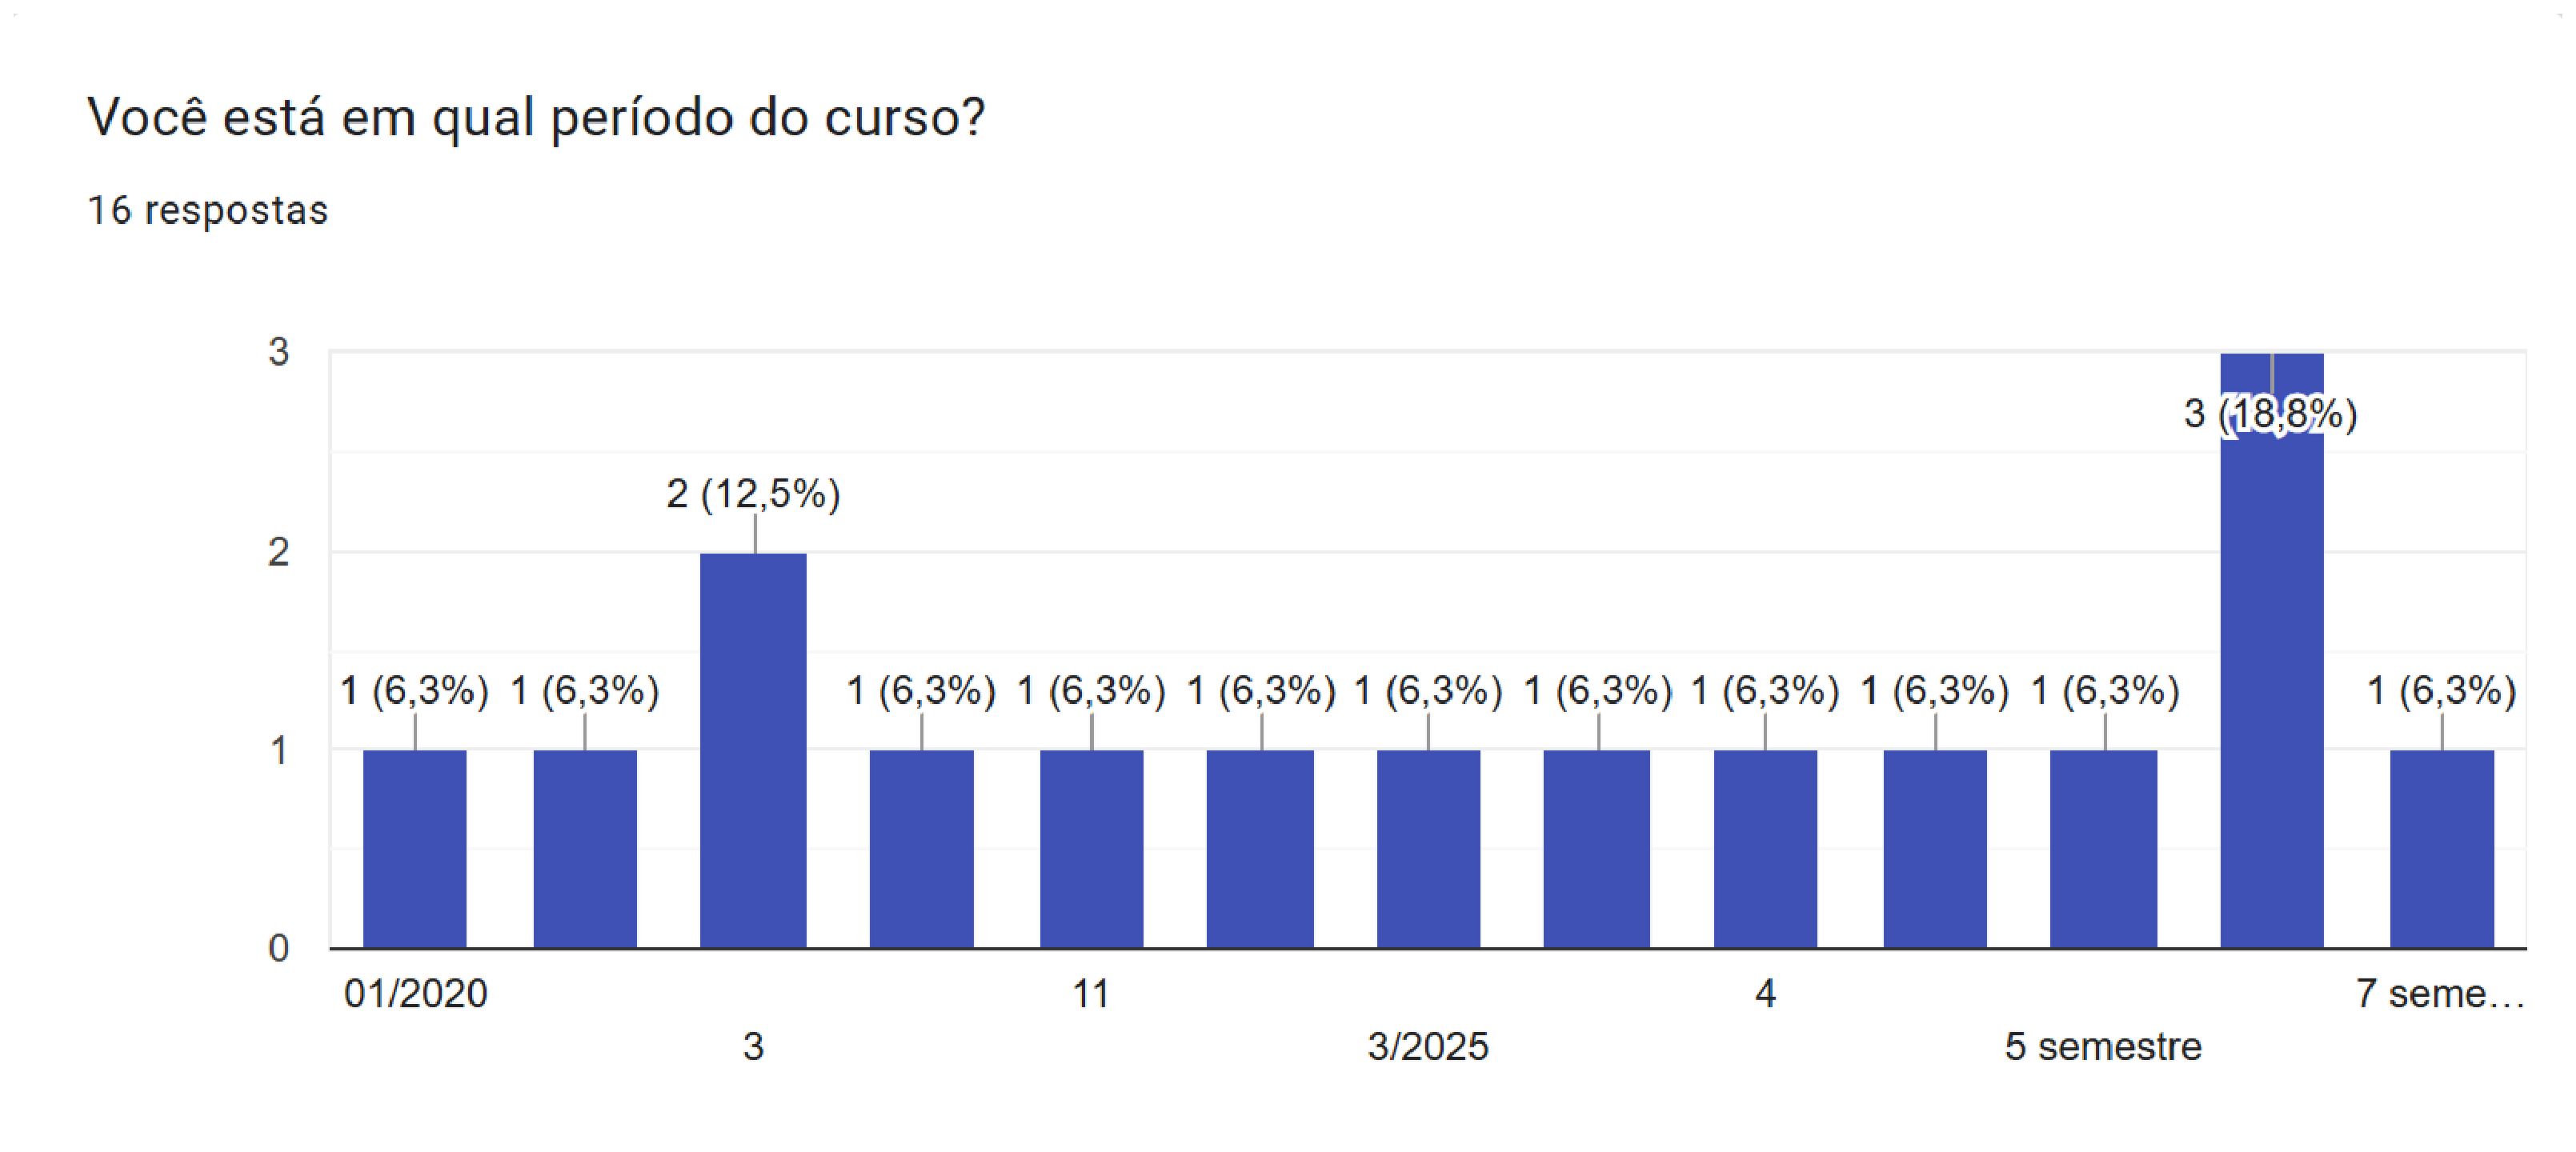
\includegraphics[width=1\linewidth]{./figuras/S1P2.eps}
	\caption{Seção 1 - Pergunta 2}
	\footnotesize Fonte: Autores.
	\label{fig07}
\end{figure}

\begin{figure}[h]
	\centering
	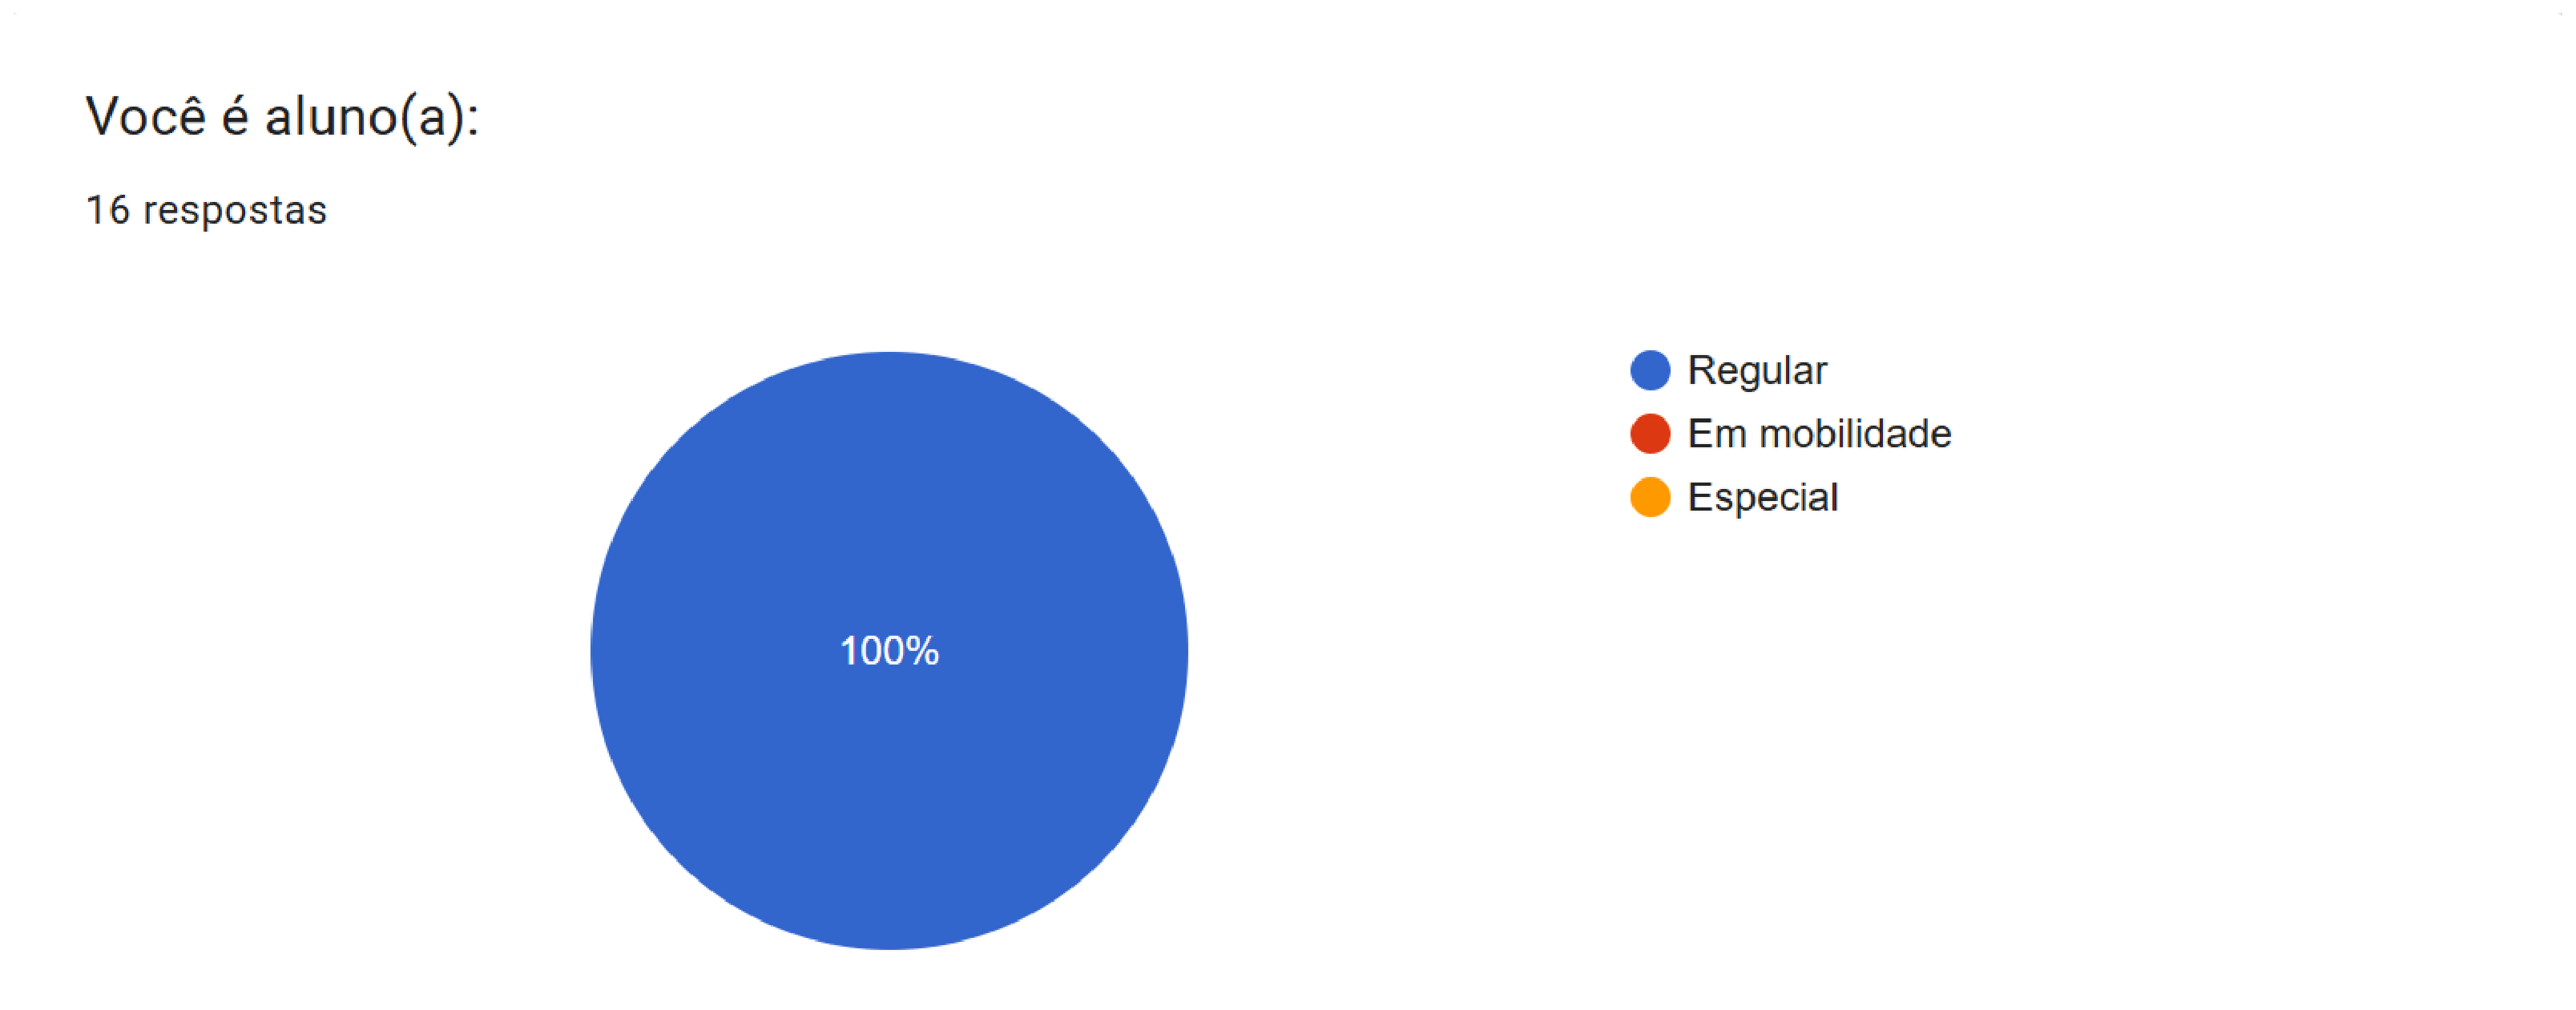
\includegraphics[width=1\linewidth]{./figuras/S1P3.eps}
	\caption{Seção 1 - Pergunta 3}
	\footnotesize Fonte: Autores.
	\label{fig08}
\end{figure}

\begin{figure}[h]
	\centering
	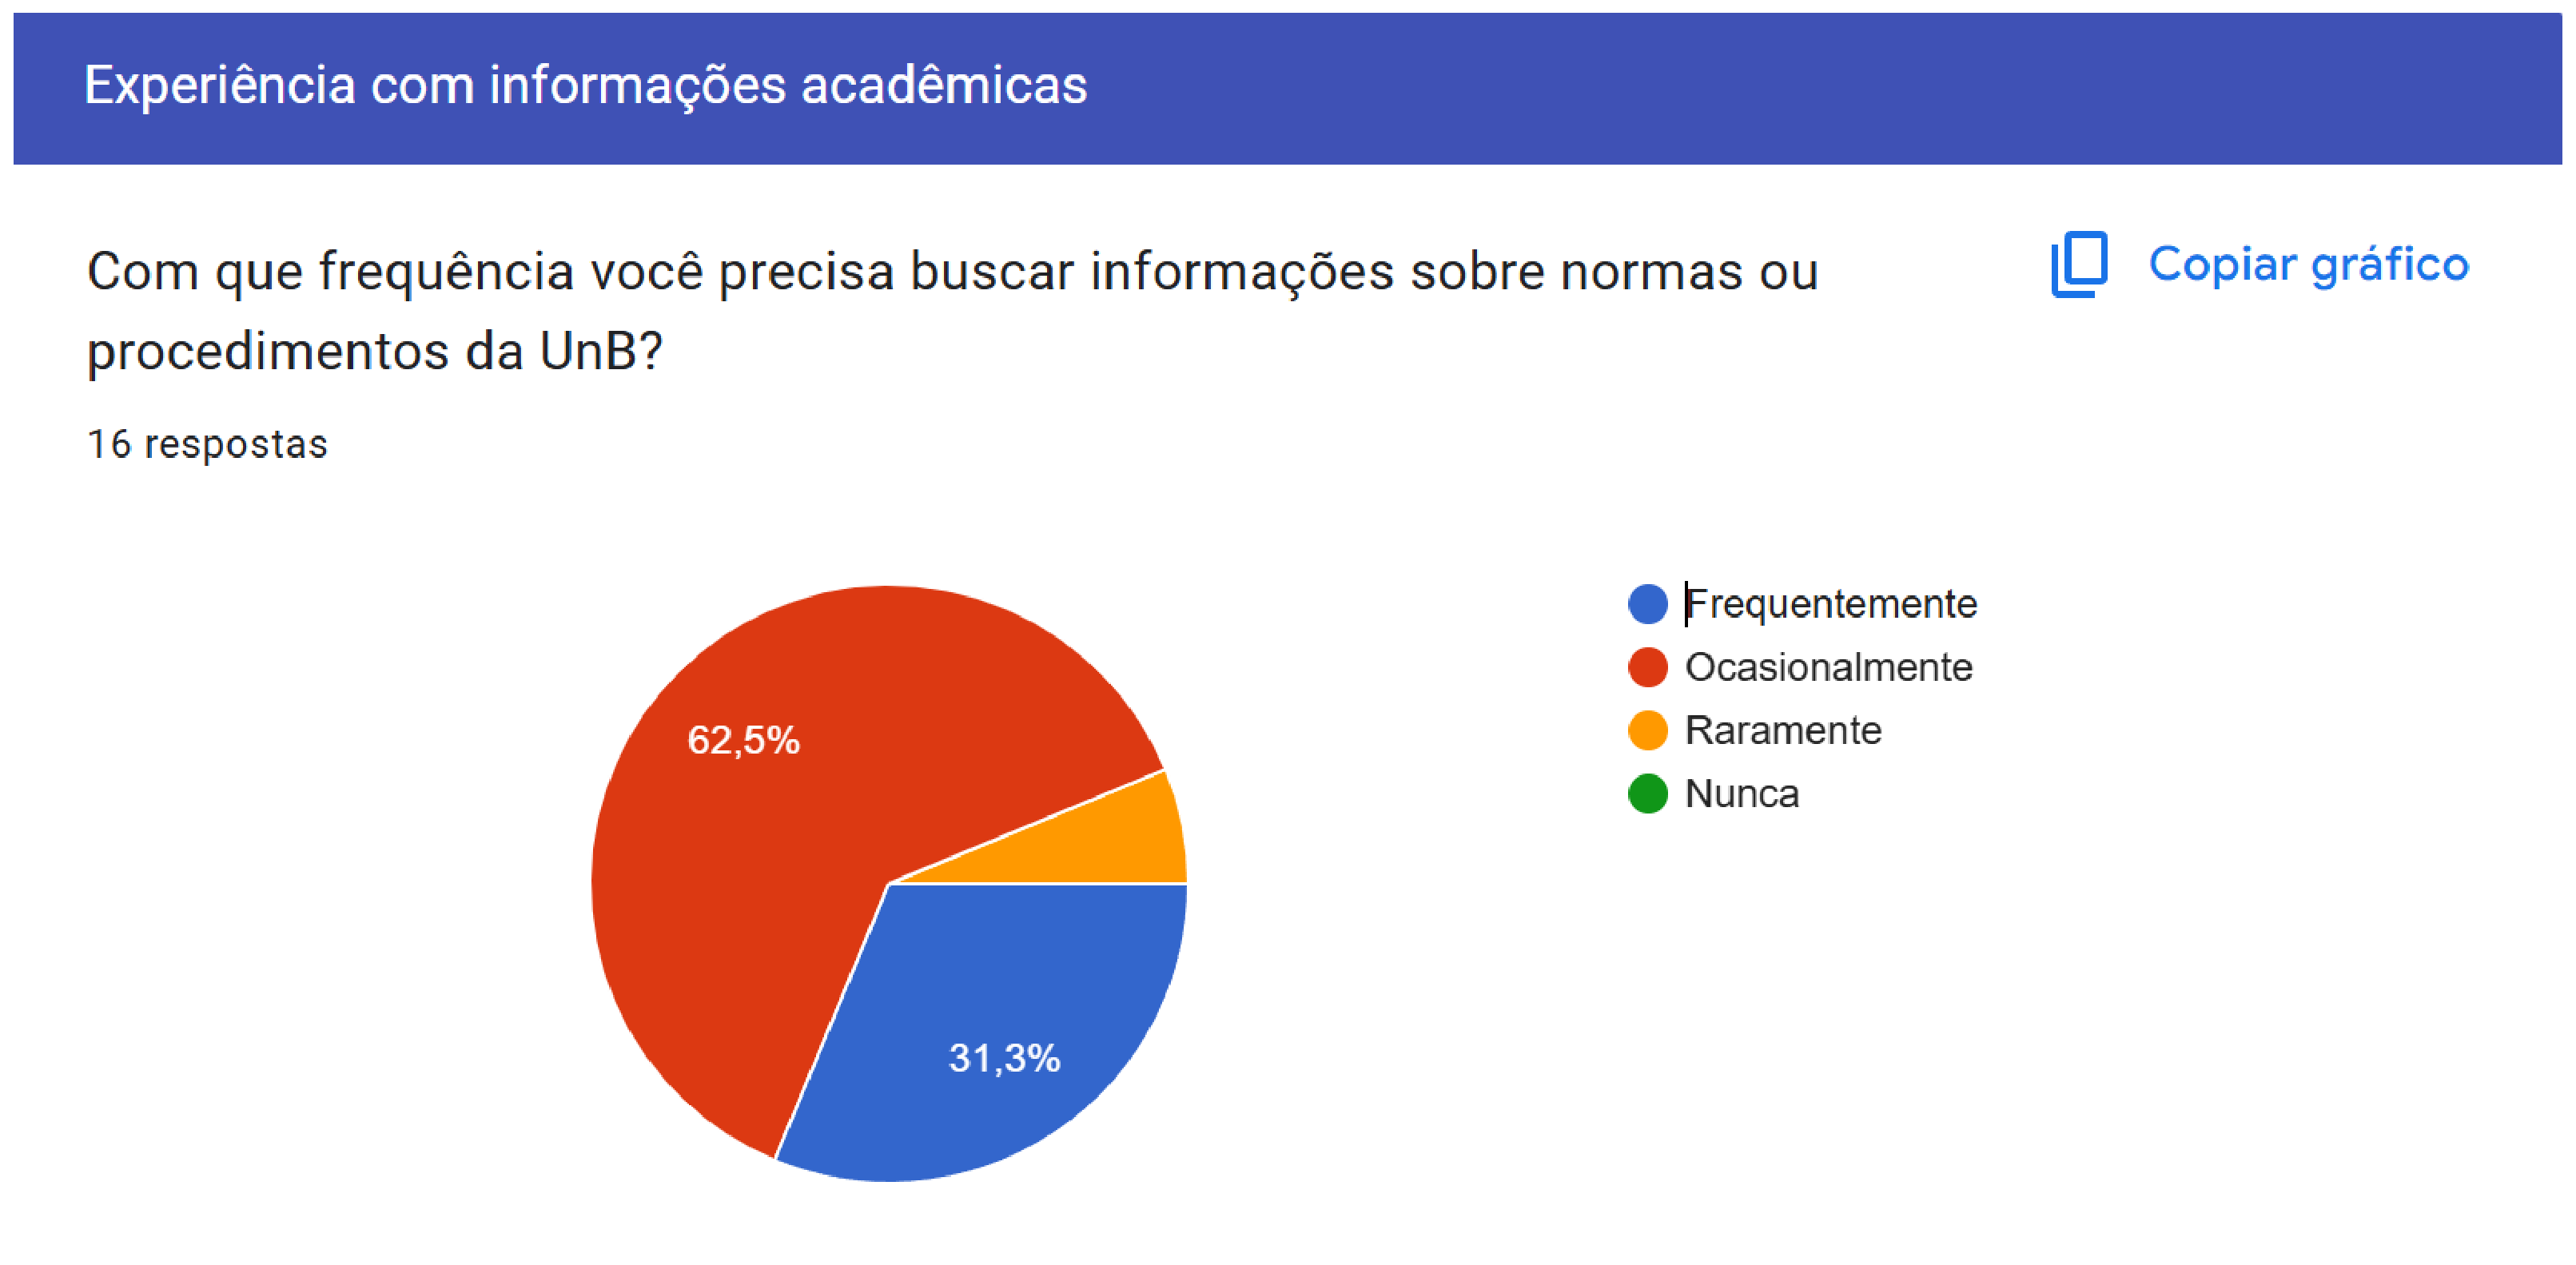
\includegraphics[width=1\linewidth]{./figuras/S2P1.eps}
	\caption{Seção 2 - Pergunta 1}
	\footnotesize Fonte: Autores.
	\label{fig09}
\end{figure}

\begin{figure}[h]
	\centering
	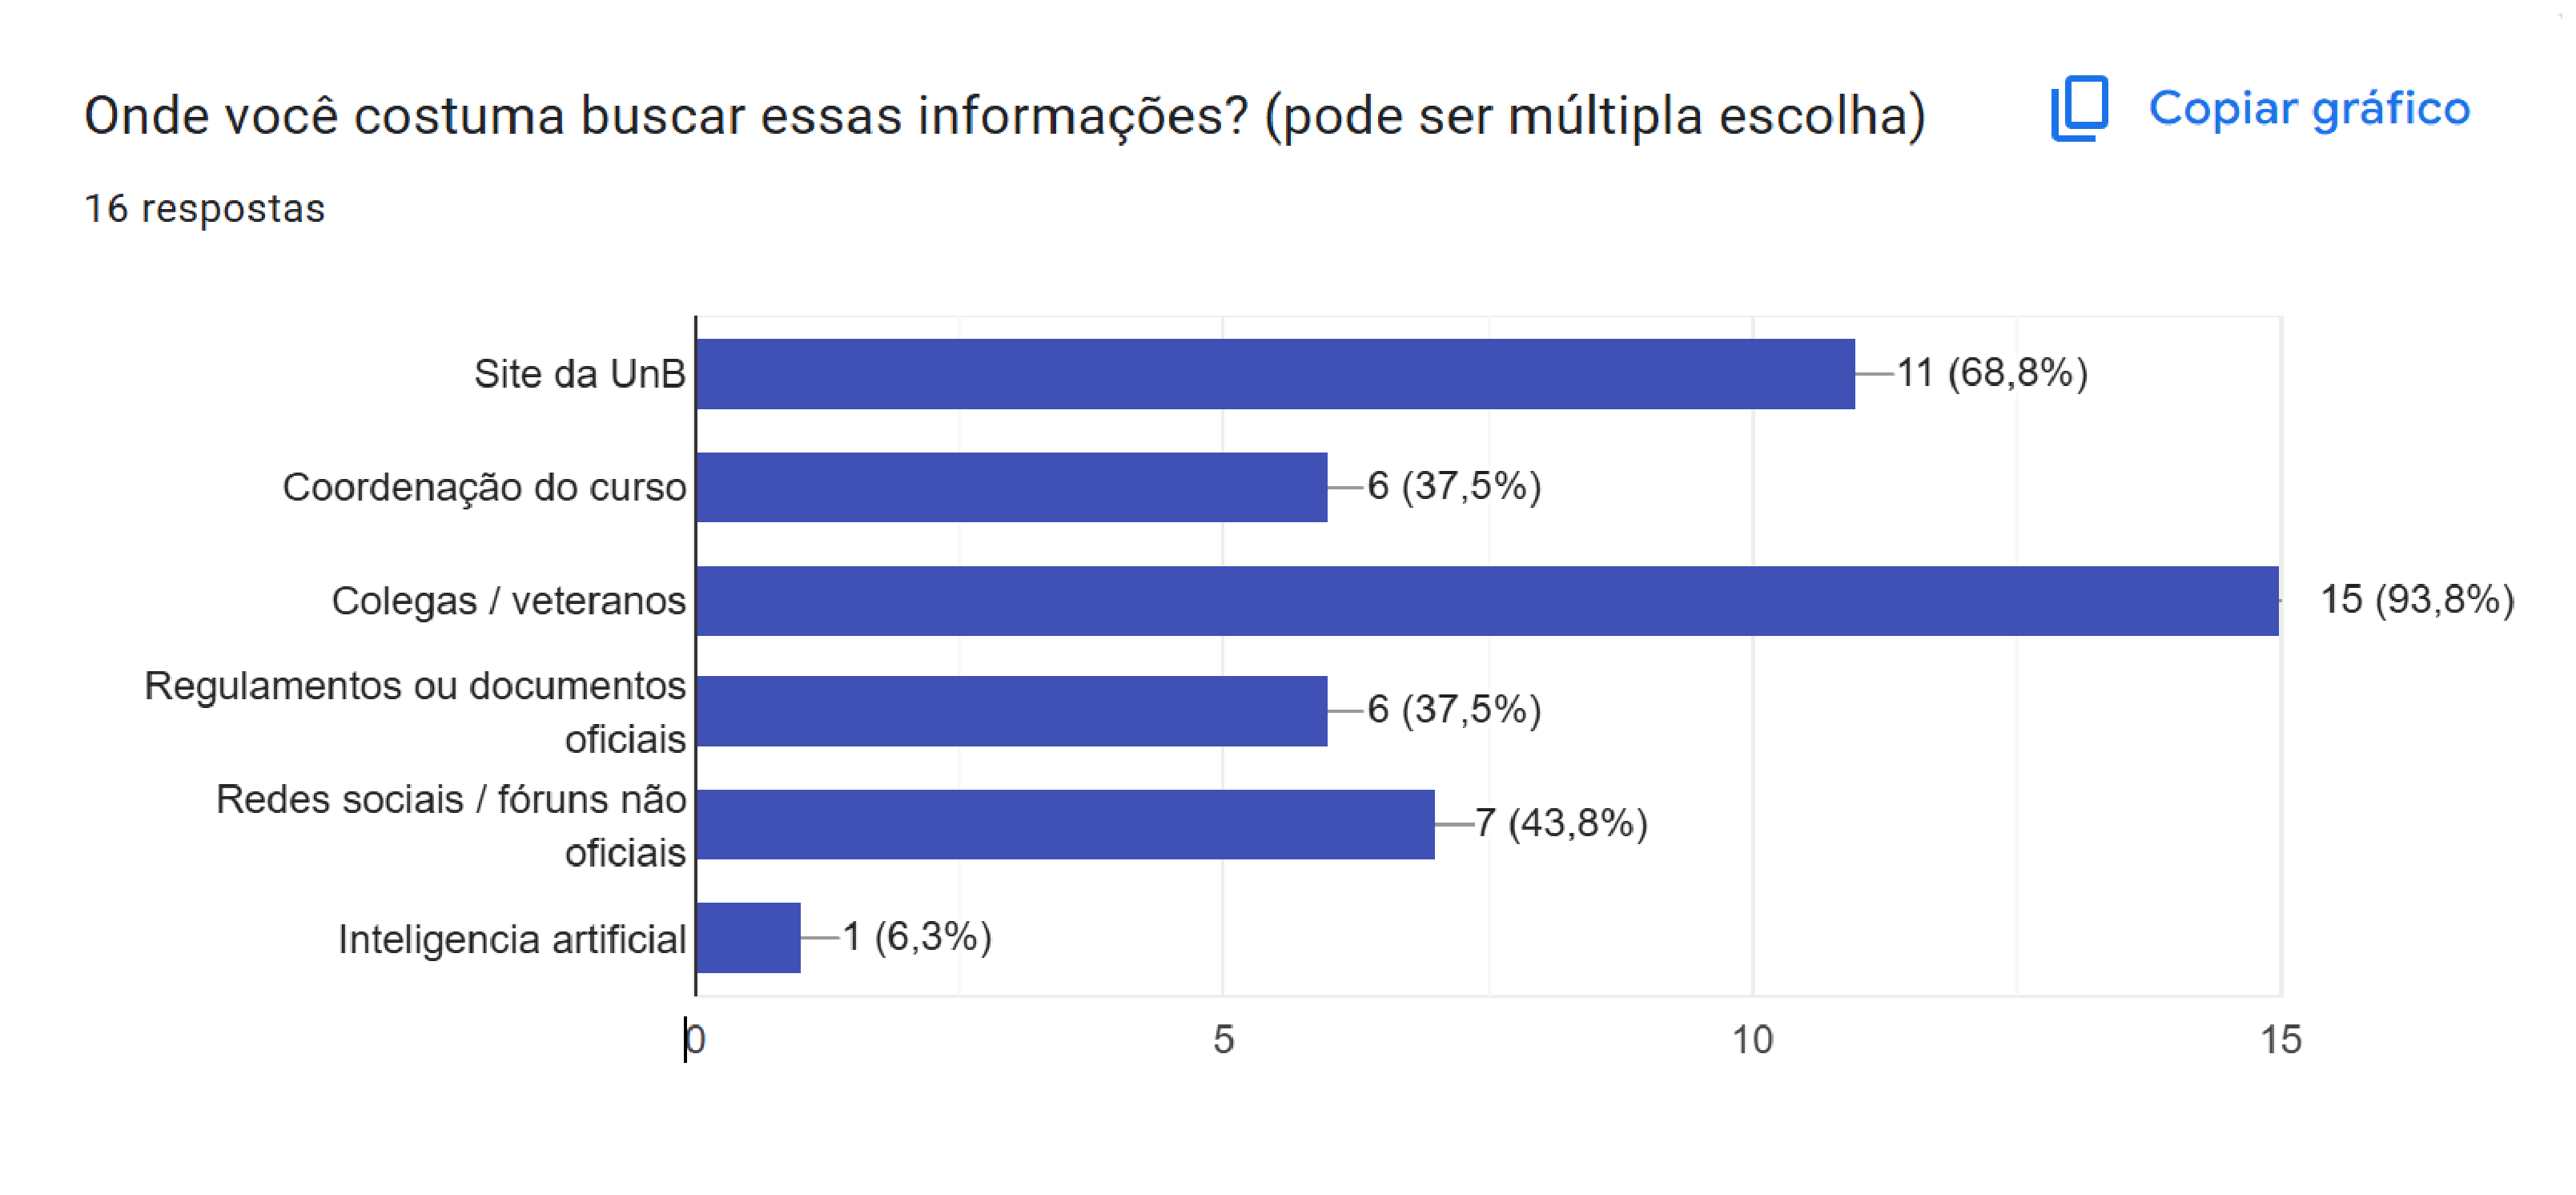
\includegraphics[width=1\linewidth]{./figuras/S2P2.eps}
	\caption{Seção 2 - Pergunta 2}
	\footnotesize Fonte: Autores.
	\label{fig10}
\end{figure}

\begin{figure}[h]
	\centering
	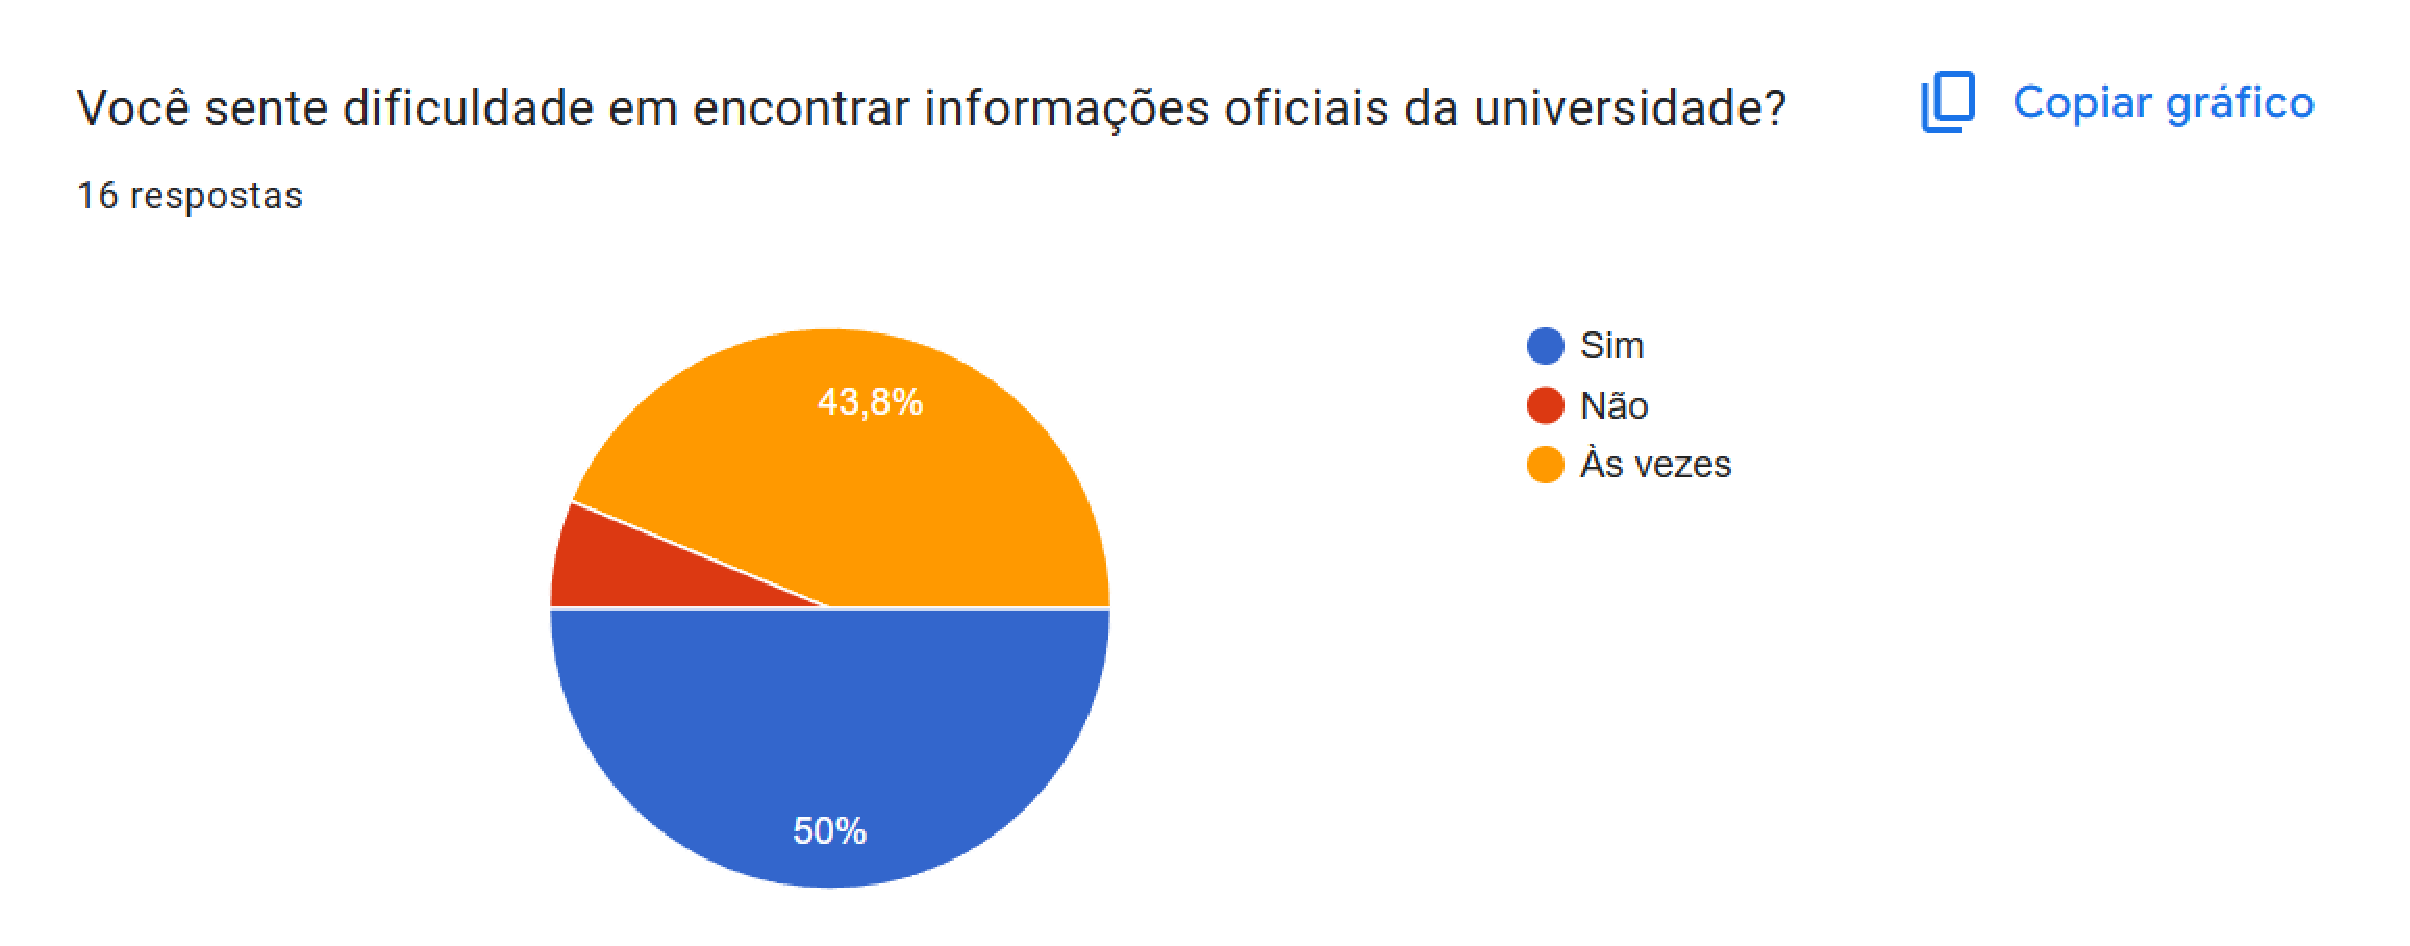
\includegraphics[width=1\linewidth]{./figuras/S2P3.eps}
	\caption{Seção 2 - Pergunta 3}
	\footnotesize Fonte: Autores.
	\label{fig11}
\end{figure}

\begin{figure}[h]
	\centering
	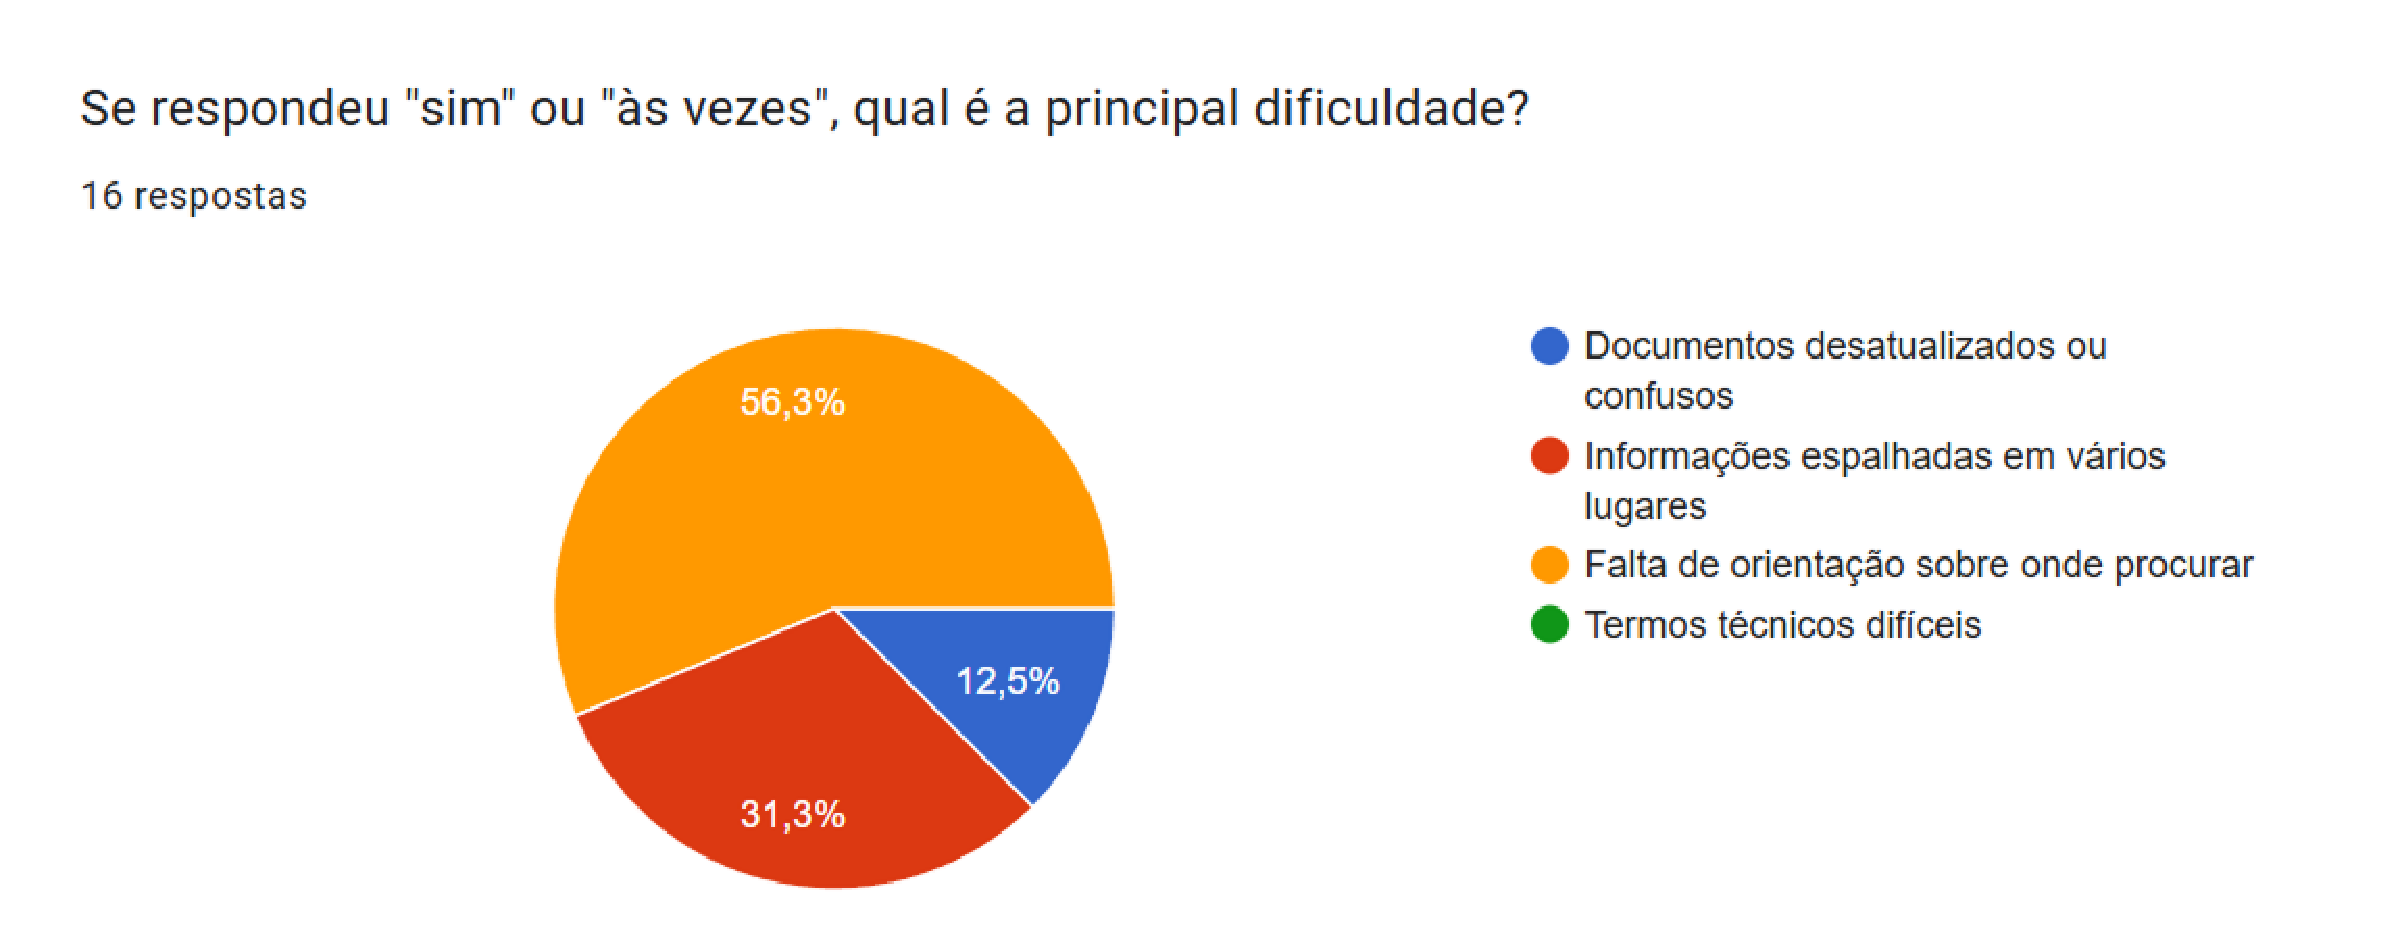
\includegraphics[width=1\linewidth]{./figuras/S2P4.eps}
	\caption{Seção 2 - Pergunta 4}
	\footnotesize Fonte: Autores.
	\label{fig12}
\end{figure}

\begin{figure}[h]
	\centering
	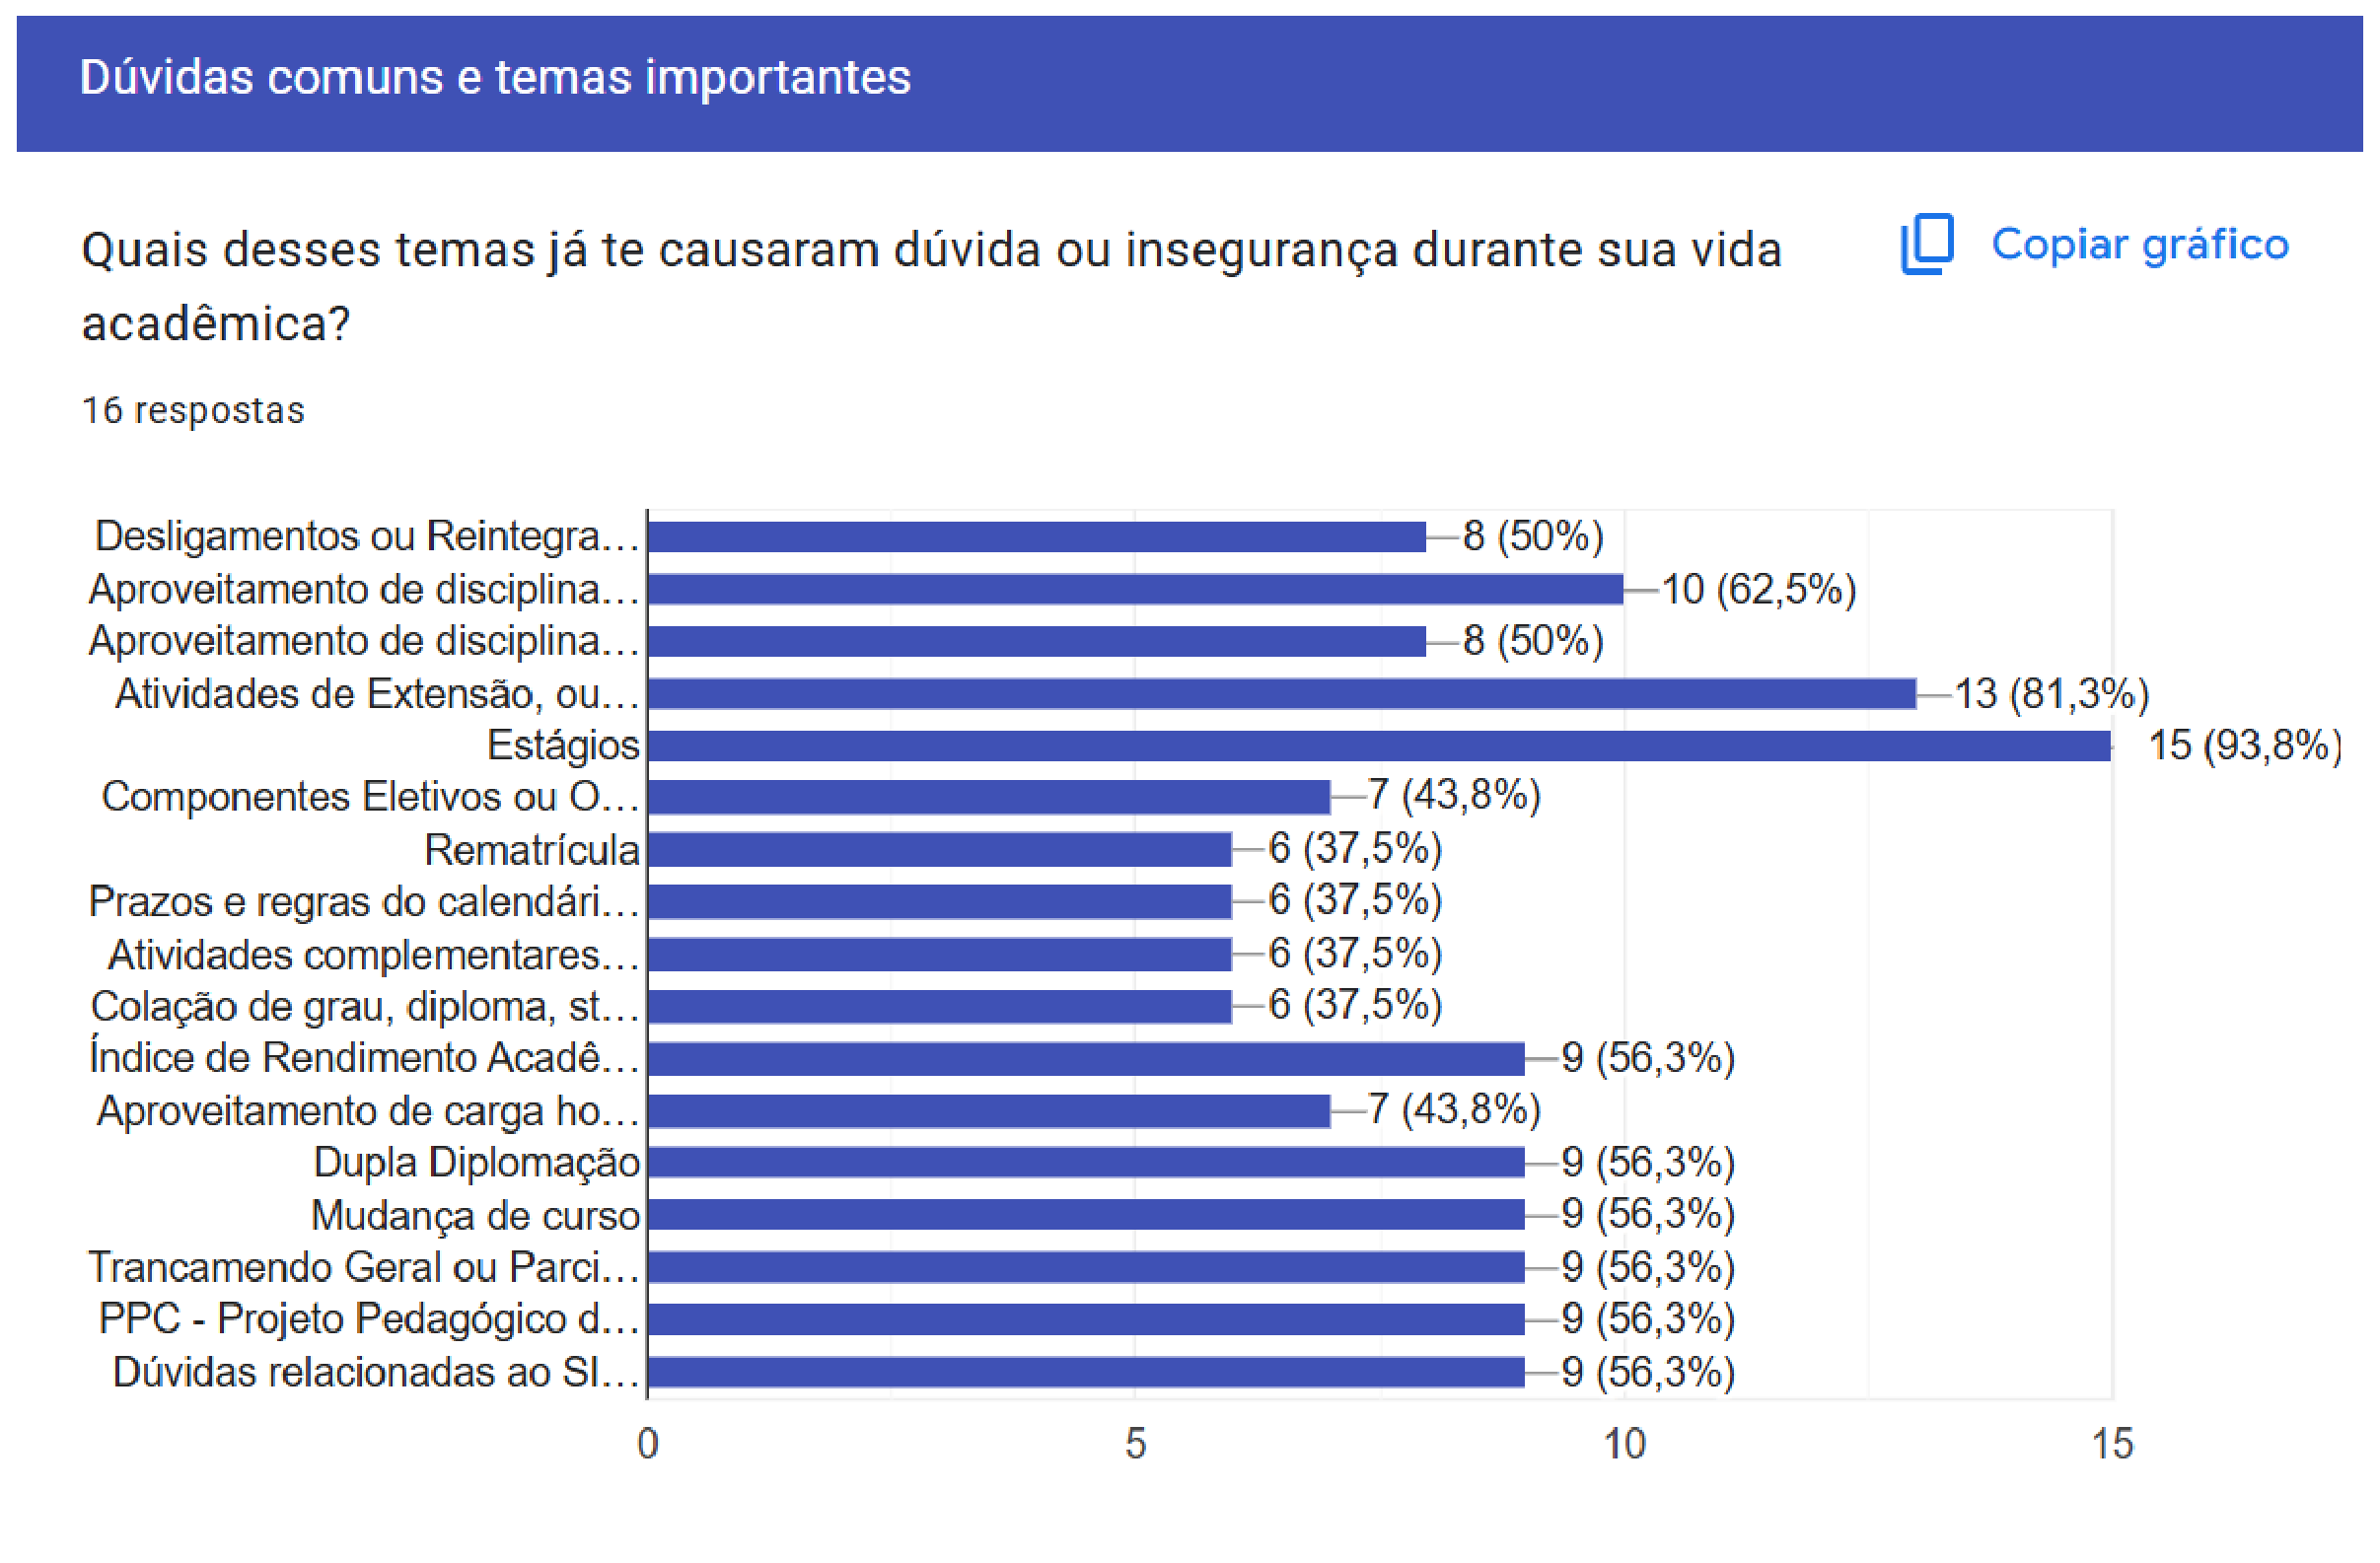
\includegraphics[width=1\linewidth]{./figuras/S3P1.eps}
	\caption{Seção 3 - Pergunta 1}
	\footnotesize Fonte: Autores.
	\label{fig13}
\end{figure}

\begin{figure}[h]
	\centering
	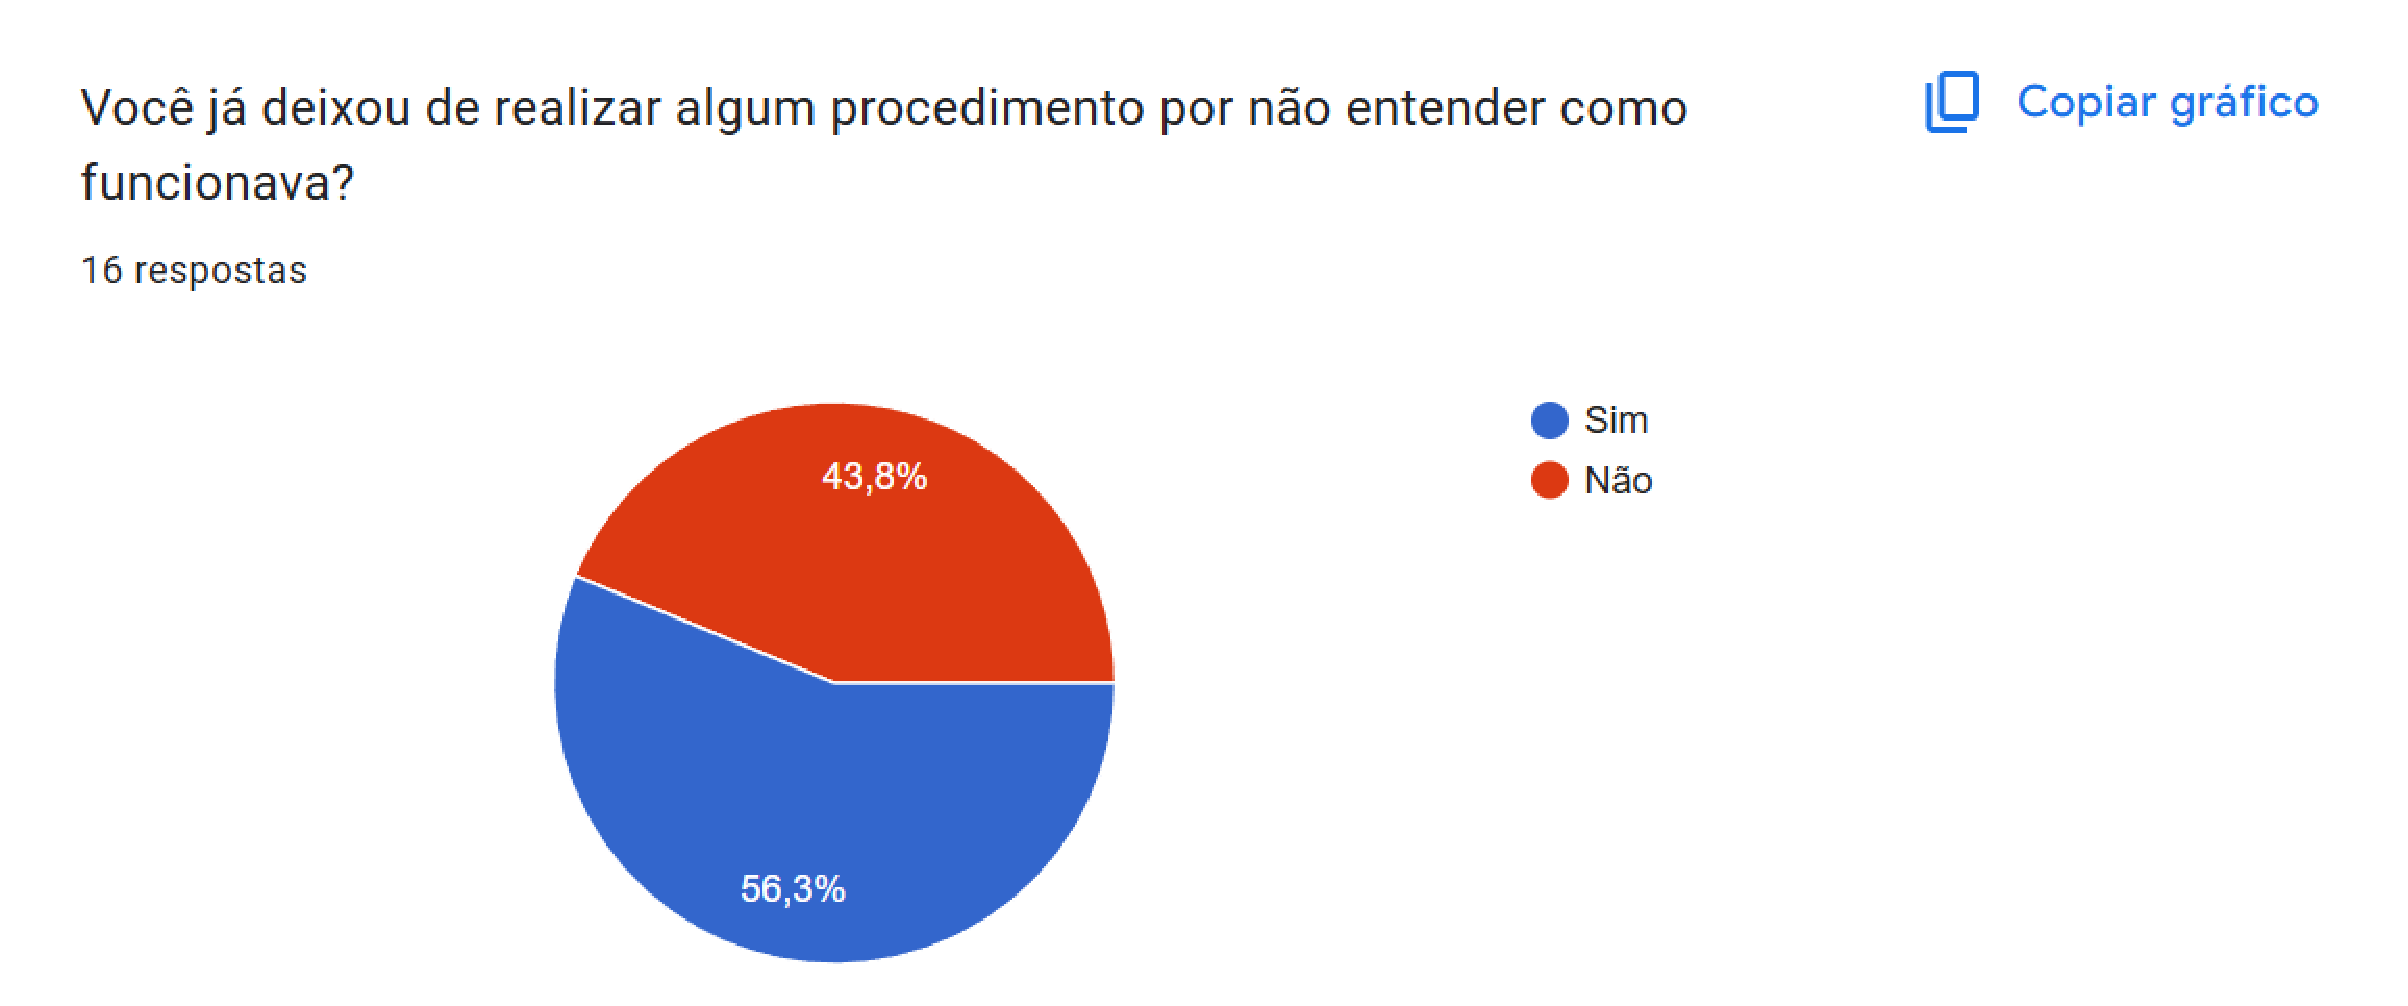
\includegraphics[width=1\linewidth]{./figuras/S3P2.eps}
	\caption{Seção 3 - Pergunta 2}
	\footnotesize Fonte: Autores.
	\label{fig14}
\end{figure}

\begin{figure}[h]
	\centering
	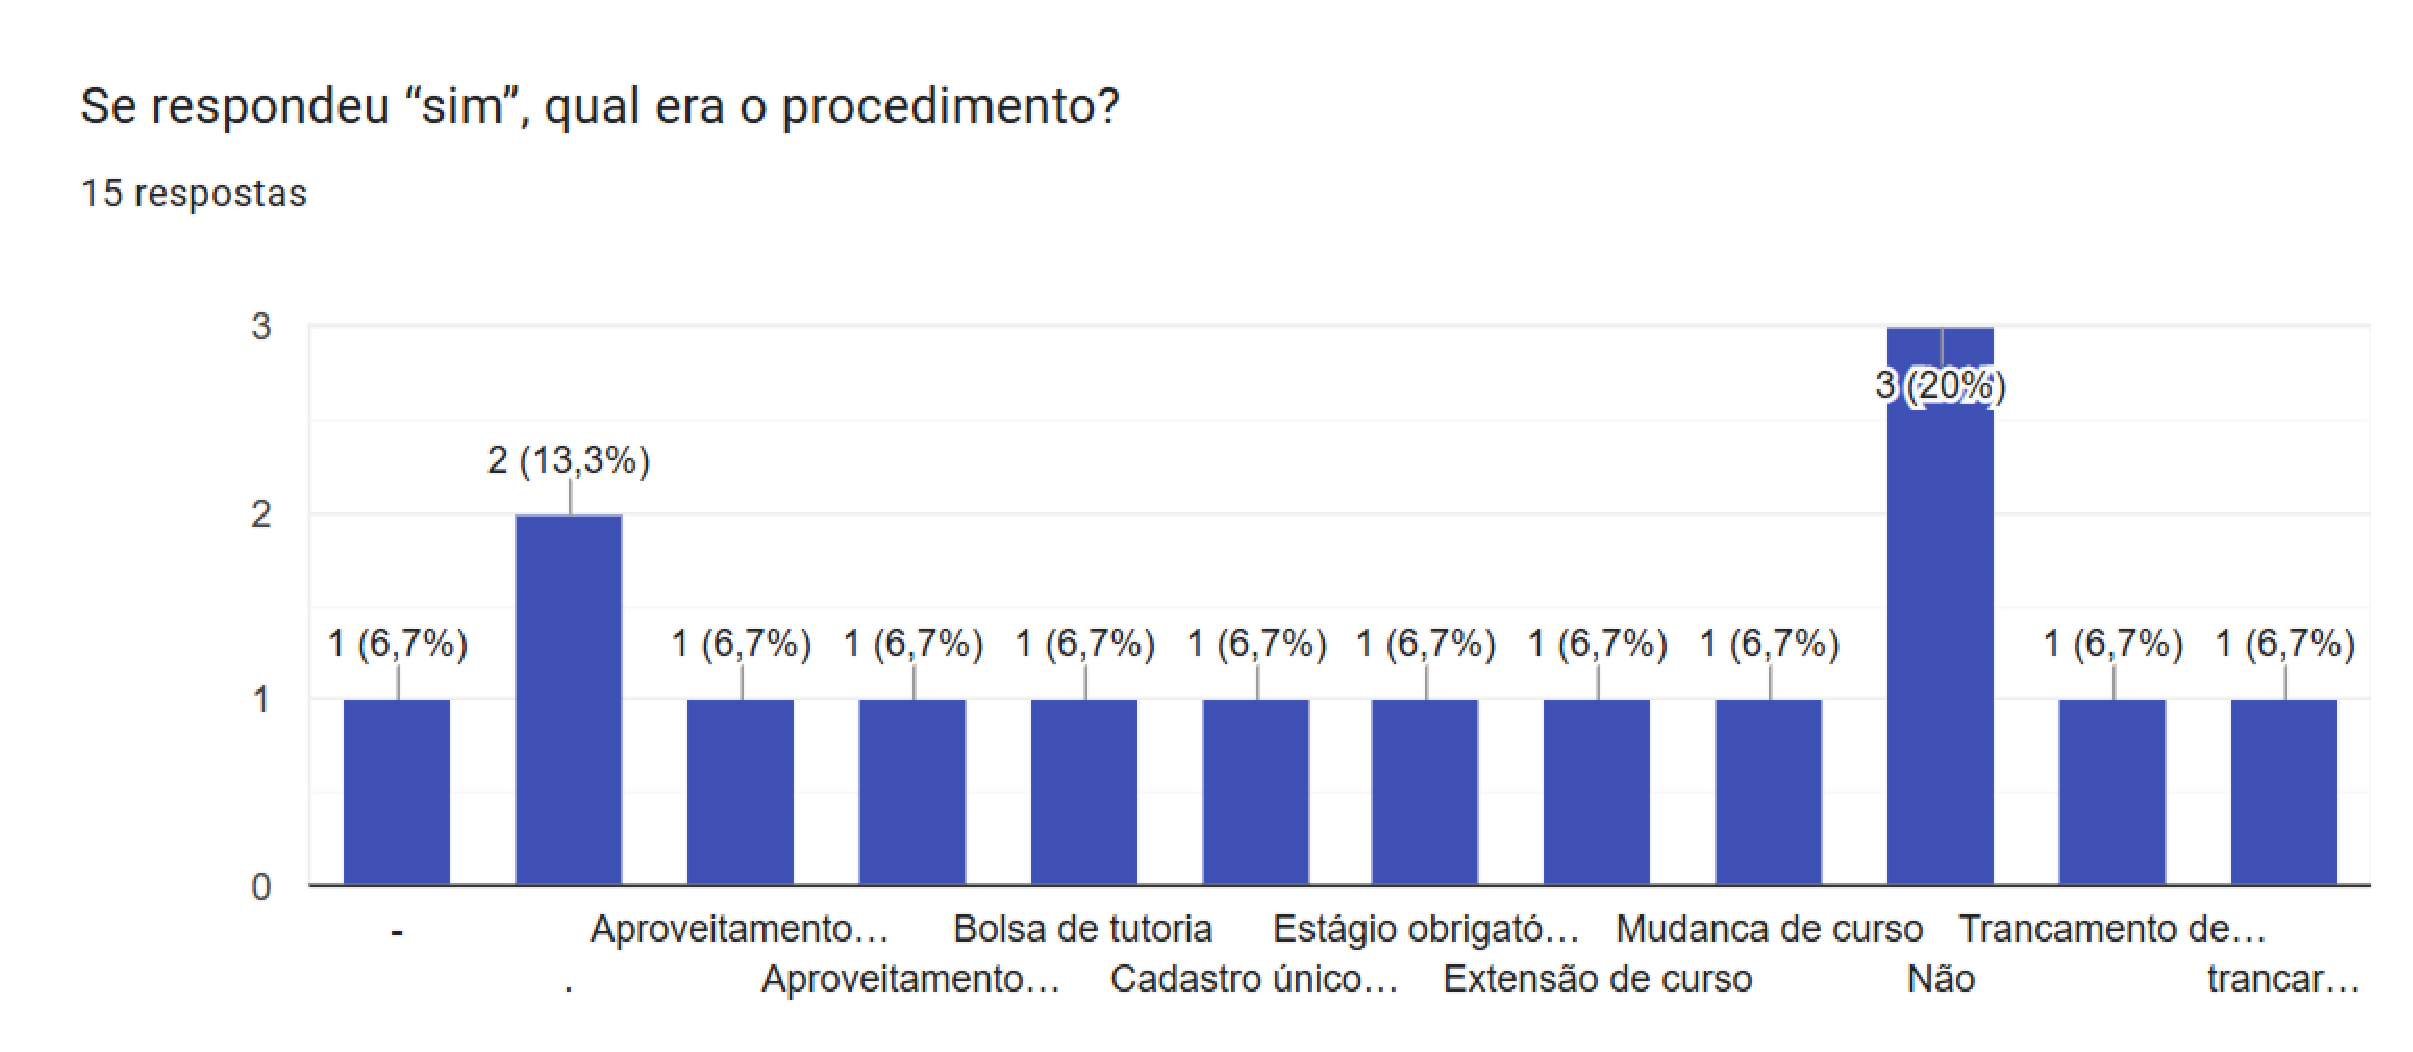
\includegraphics[width=1\linewidth]{./figuras/S3P3.eps}
	\caption{Seção 3 - Pergunta 3}
	\footnotesize Fonte: Autores.
	\label{fig15}
\end{figure}

\begin{figure}[h]
	\centering
	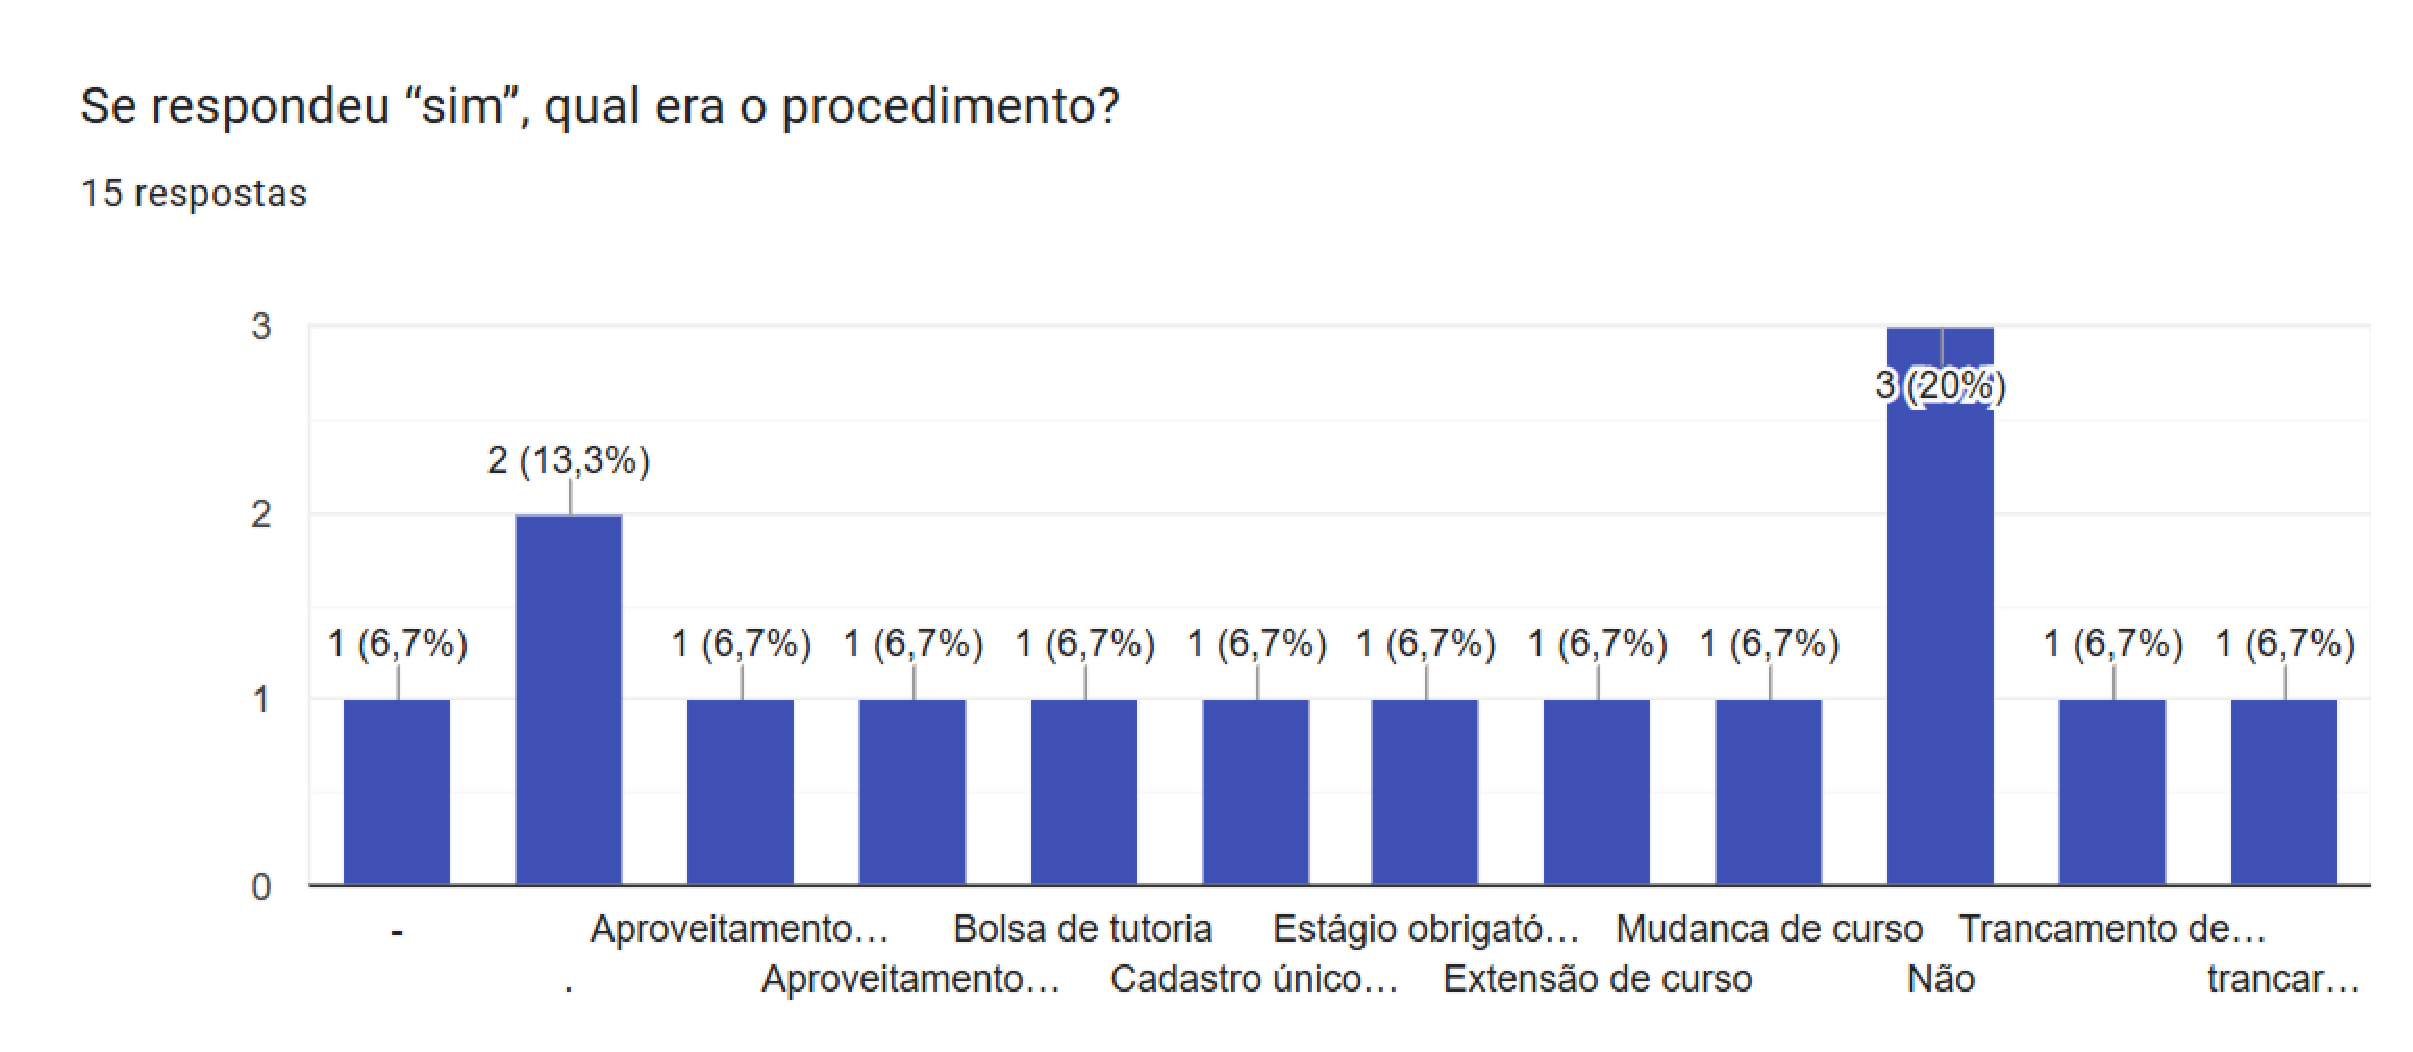
\includegraphics[width=1\linewidth]{./figuras/S3P3.eps}
	\caption{Seção 3 - Pergunta 3}
	\footnotesize Fonte: Autores.
	\label{fig16}
\end{figure}

\begin{figure}[h]
	\centering
	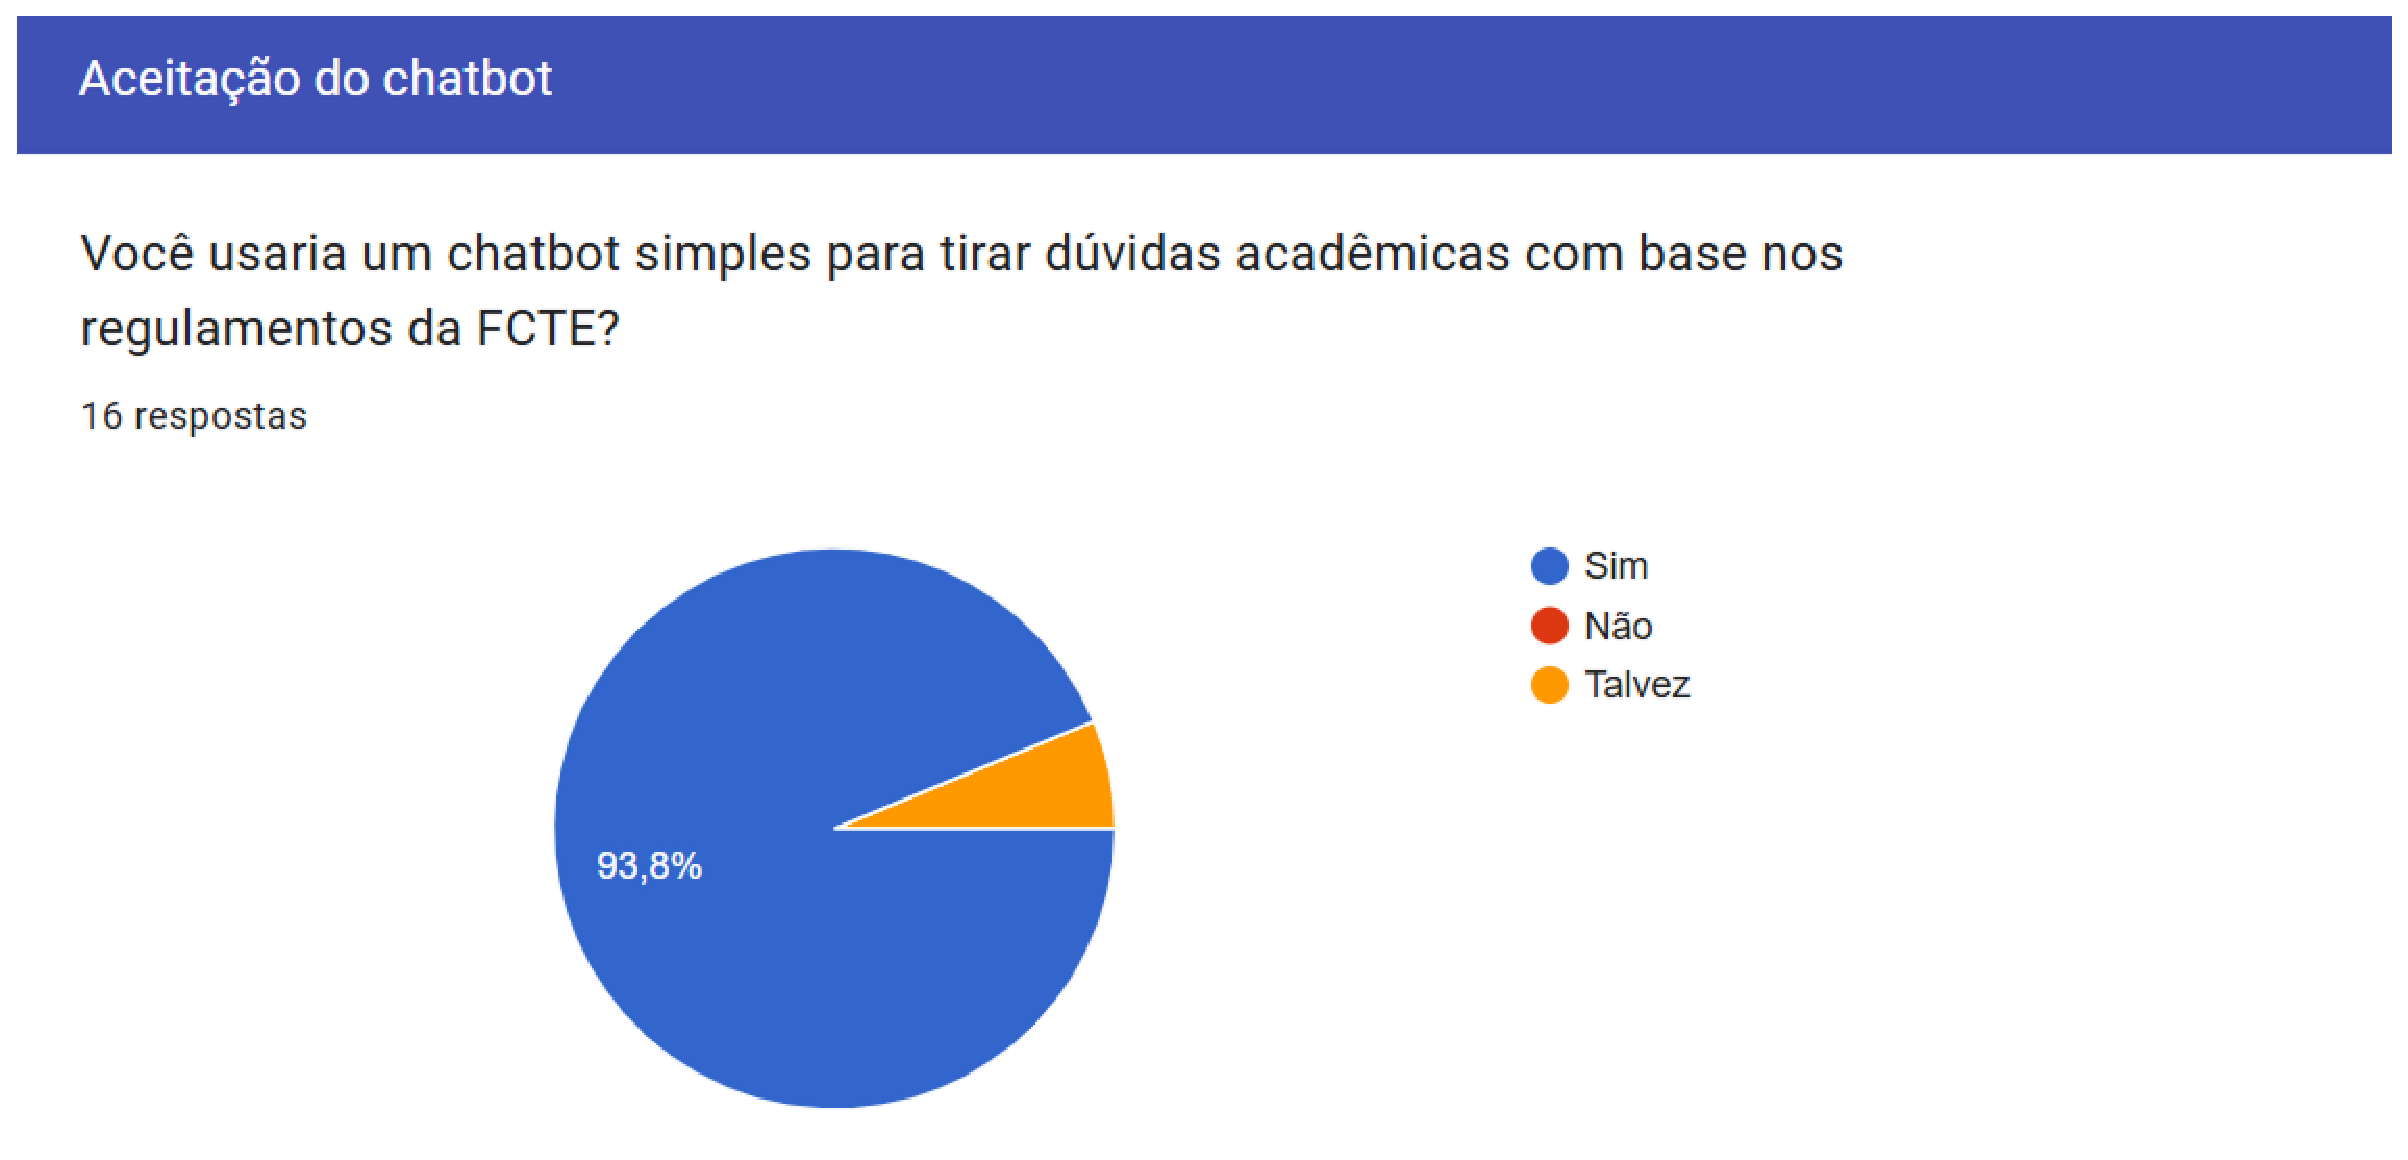
\includegraphics[width=1\linewidth]{./figuras/S4P1.eps}
	\caption{Seção 4 - Pergunta 1}
	\footnotesize Fonte: Autores.
	\label{fig17}
\end{figure}

\begin{figure}[h]
	\centering
	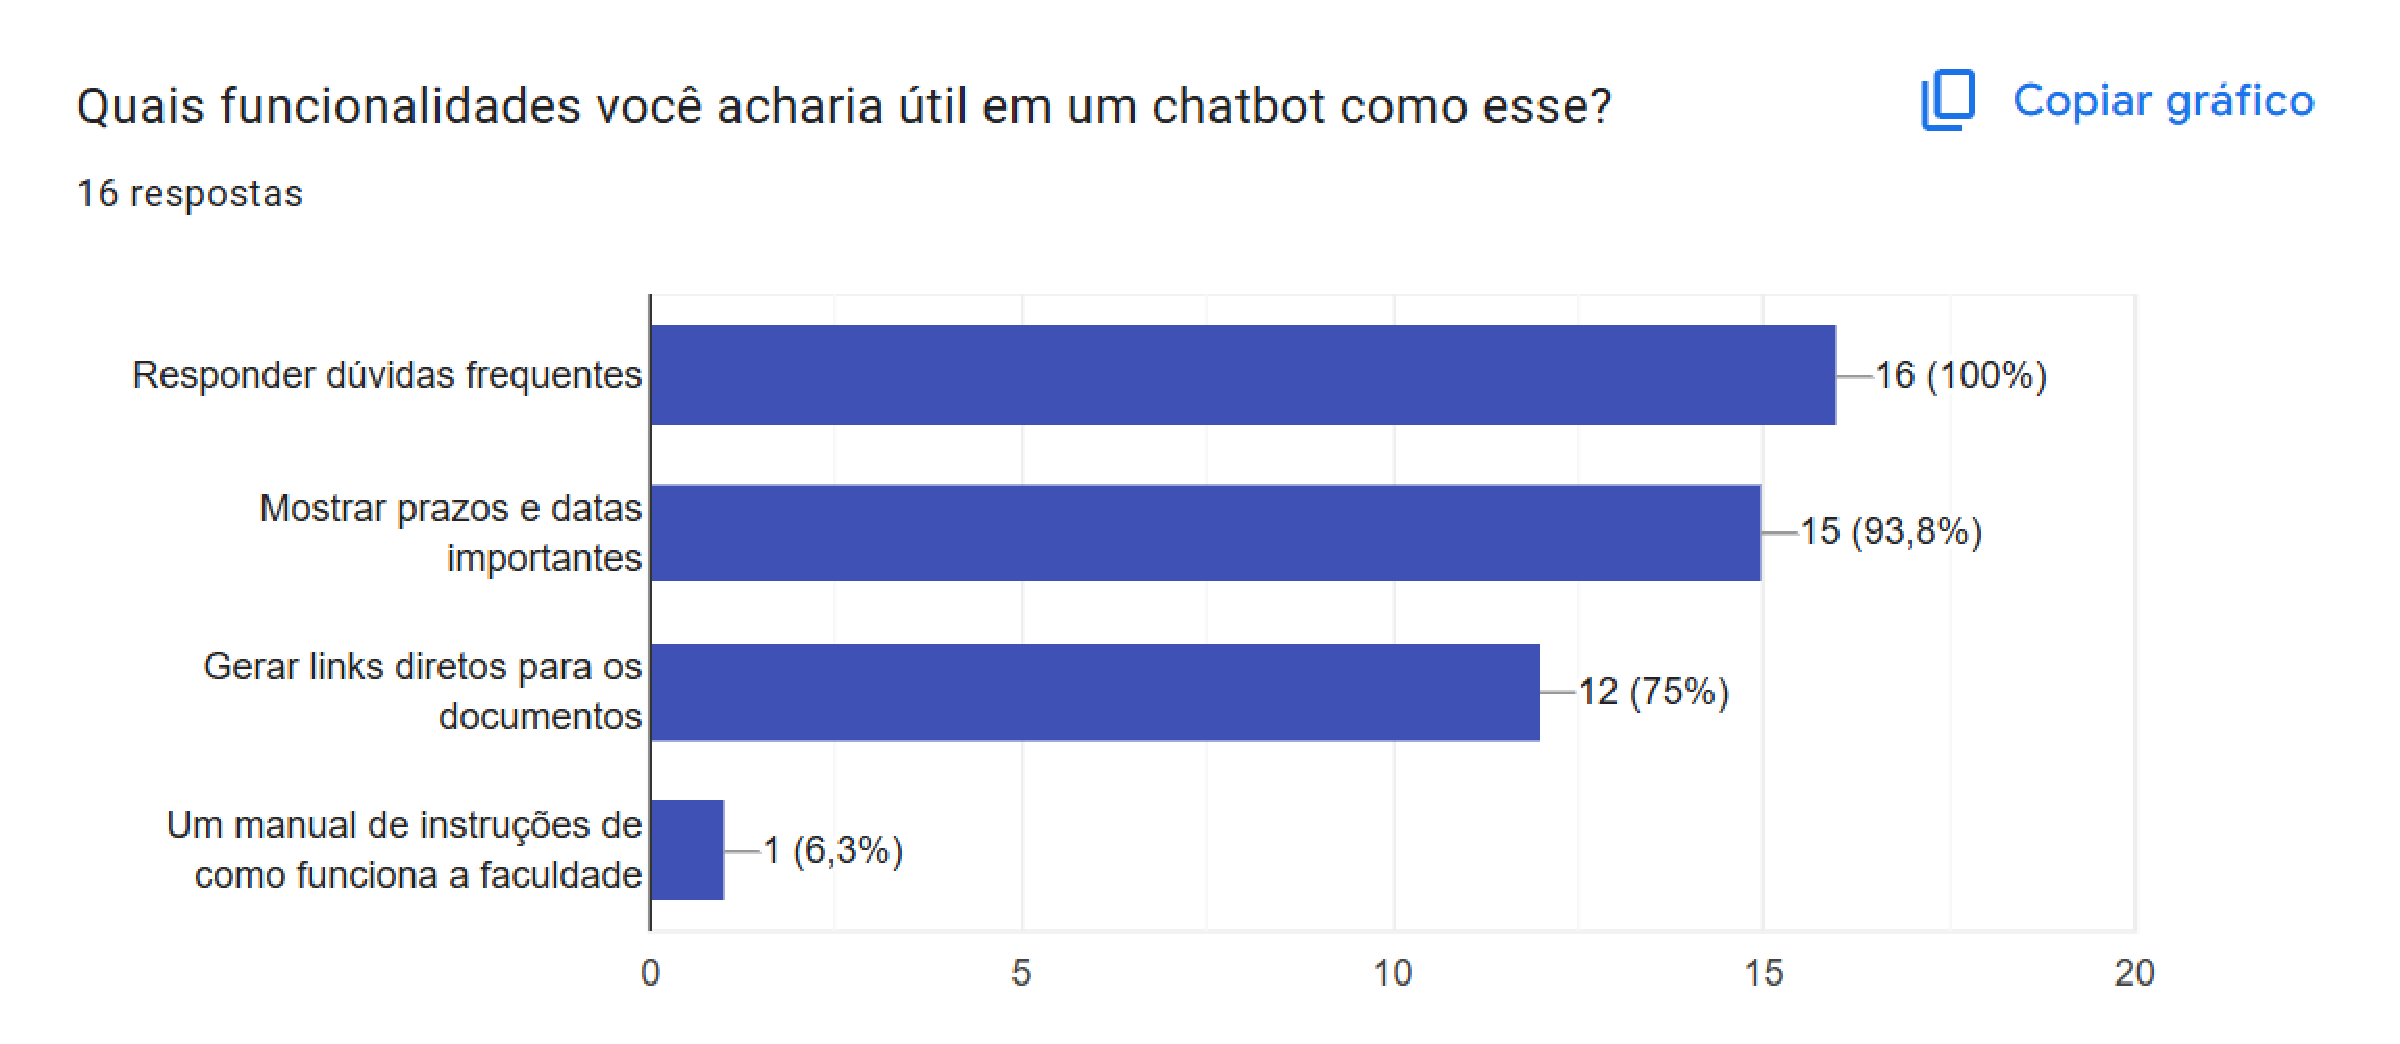
\includegraphics[width=1\linewidth]{./figuras/S4P2.eps}
	\caption{Seção 4 - Pergunta 2}
	\footnotesize Fonte: Autores.
	\label{fig18}
\end{figure}

\begin{figure}[h]
	\centering
	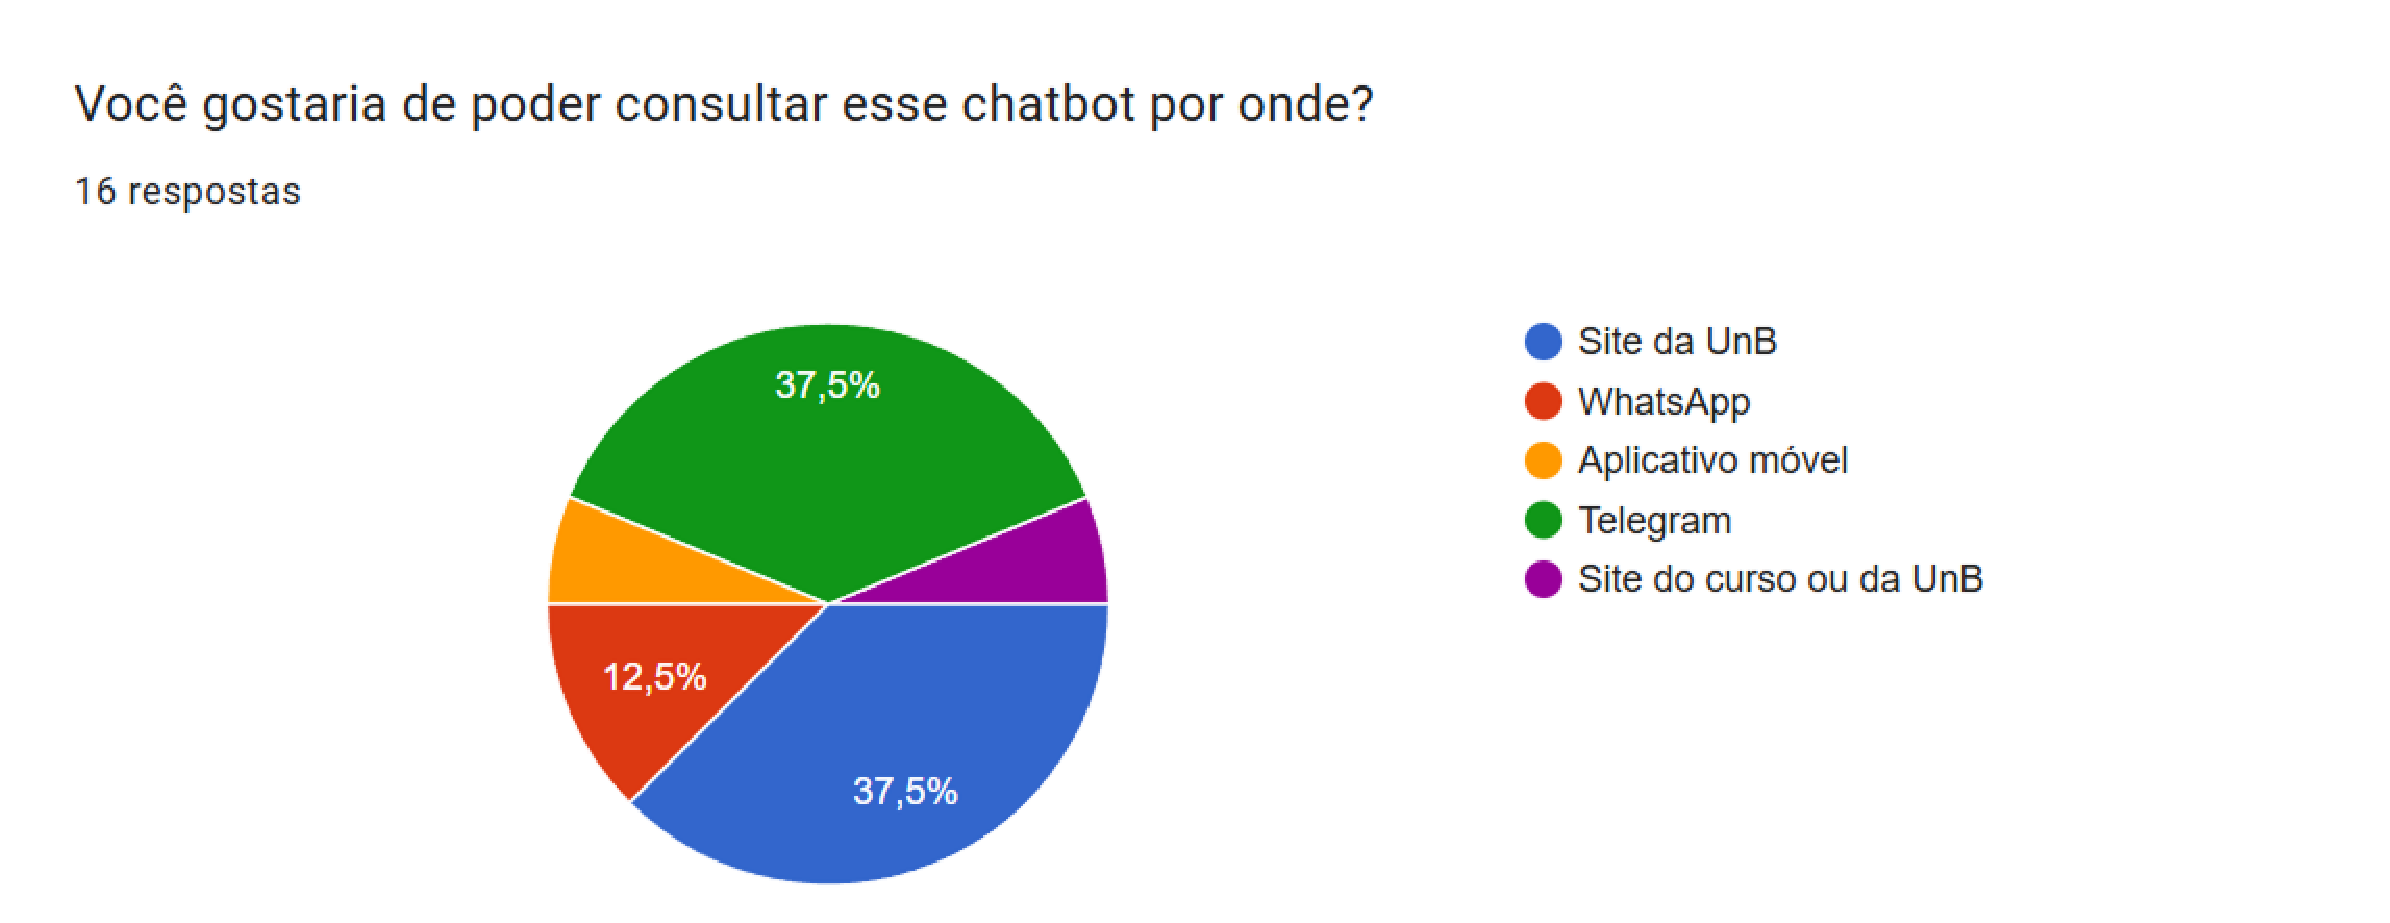
\includegraphics[width=1\linewidth]{./figuras/S4P3.eps}
	\caption{Seção 4 - Pergunta 3}
	\footnotesize Fonte: Autores.
	\label{fig19}
\end{figure}

\begin{figure}[h]
	\centering
	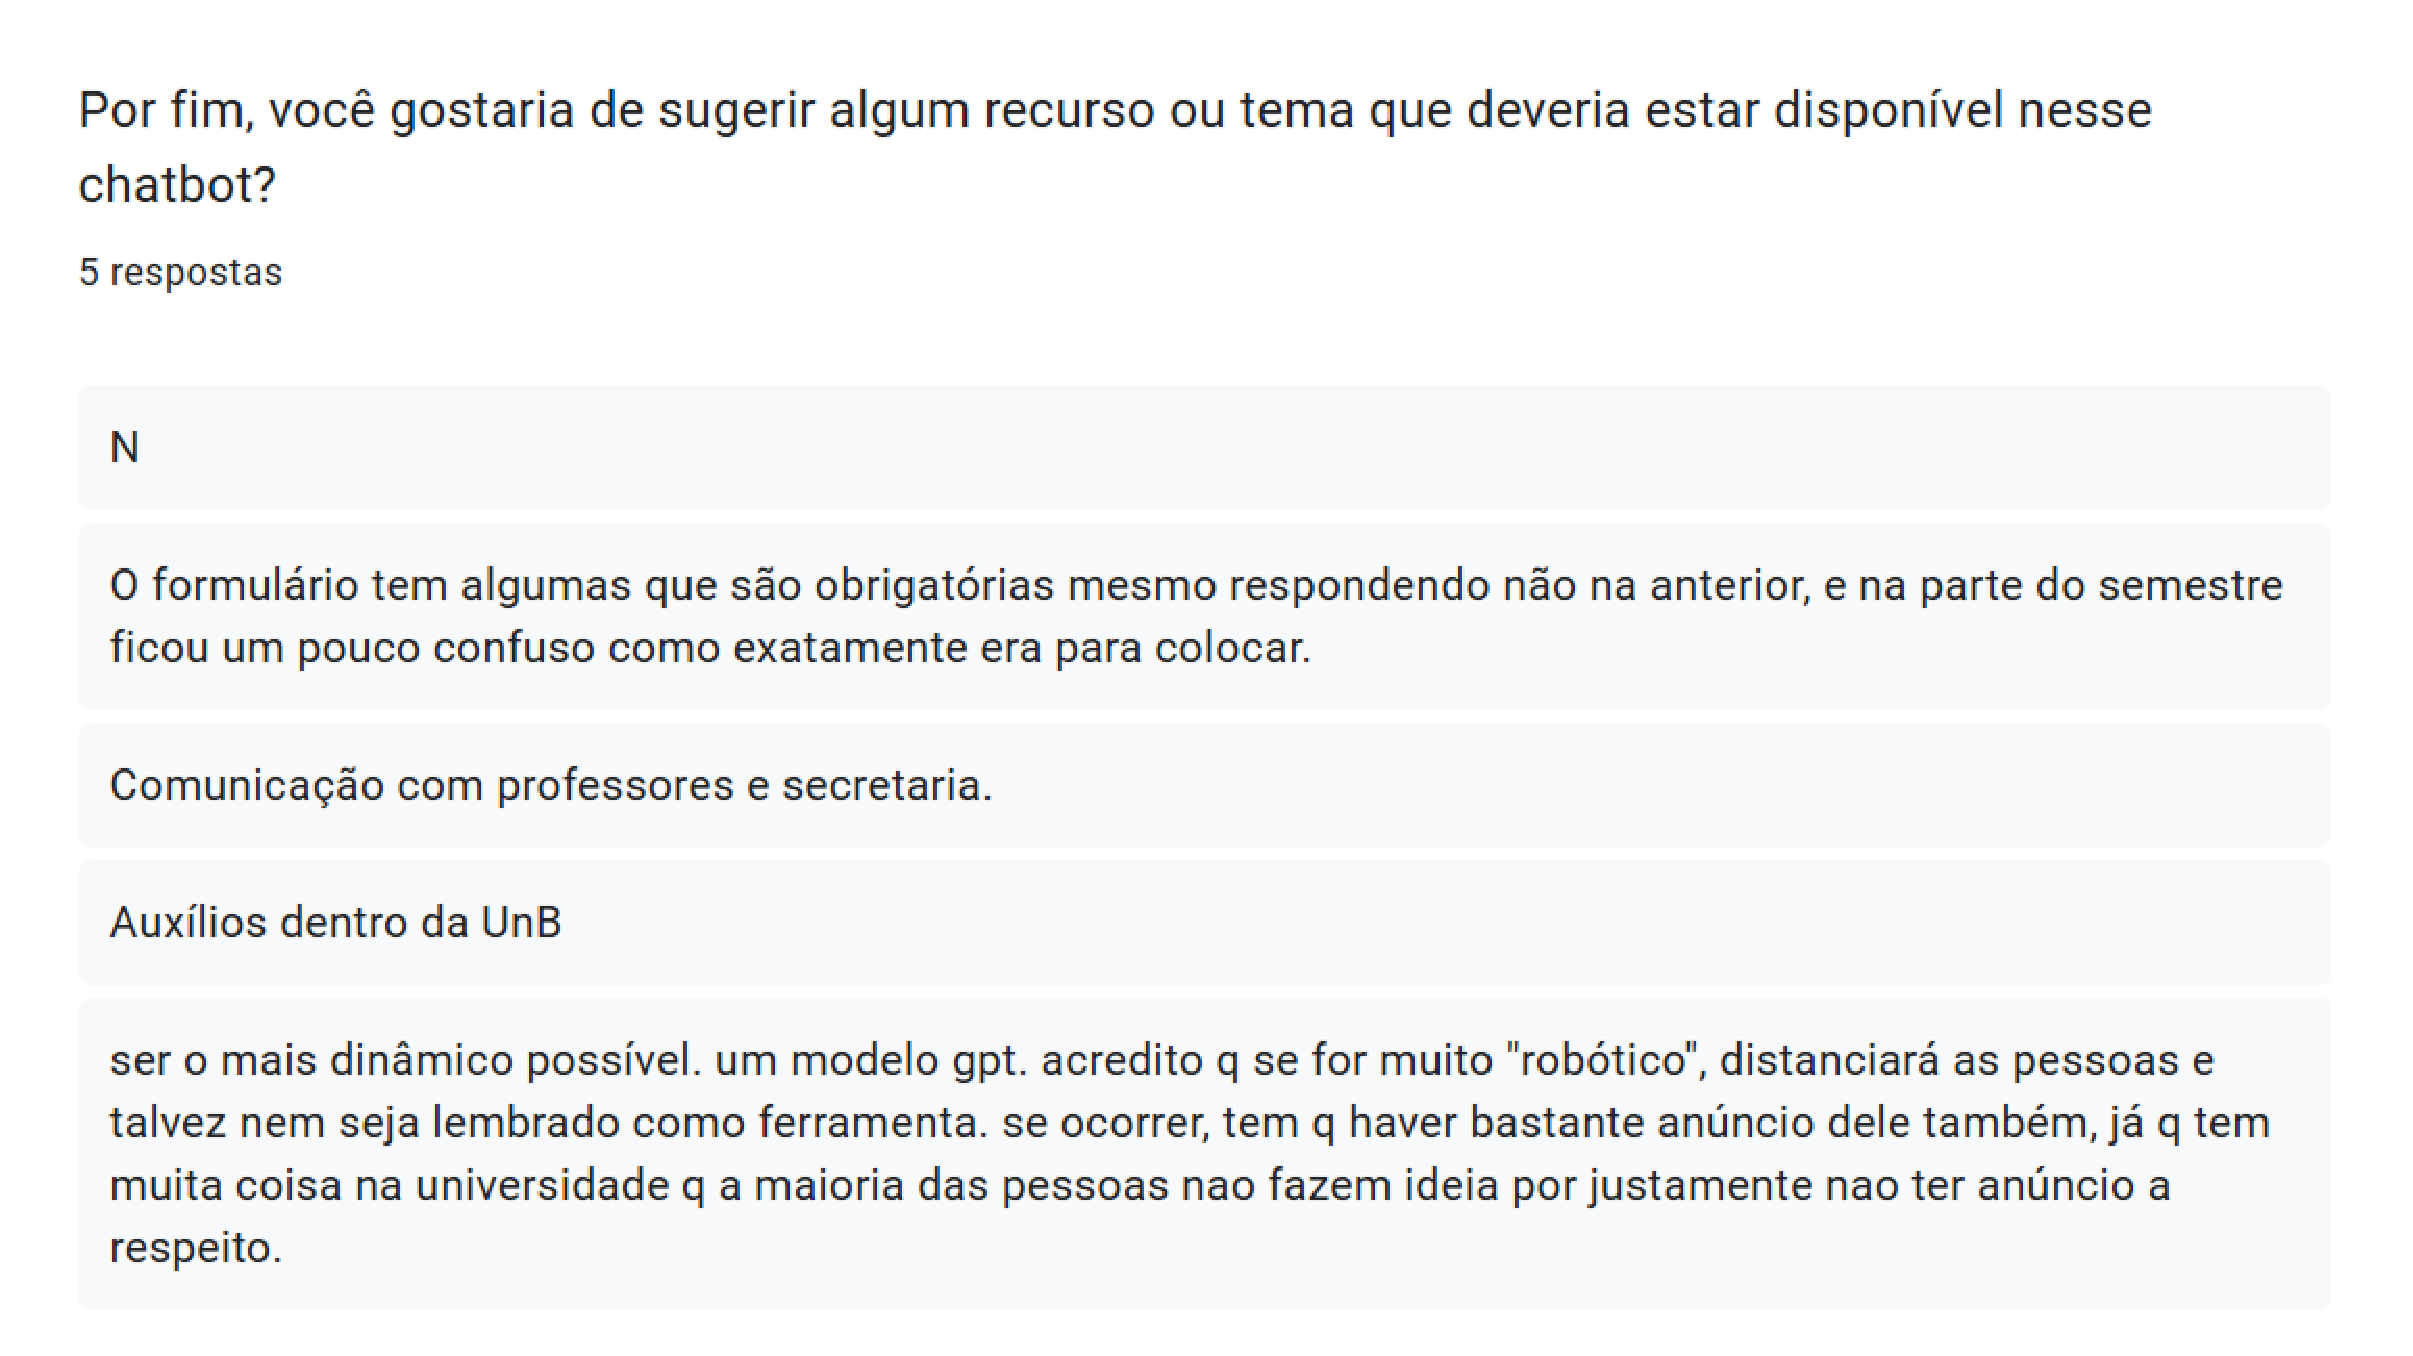
\includegraphics[width=1\linewidth]{./figuras/S4P4.eps}
	\caption{Seção 4 - Pergunta 4}
	\footnotesize Fonte: Autores.
	\label{fig20}
\end{figure}

\end{apendicesenv}
